%%**************************************************************
%% Vorlage fuer Bachelorarbeiten (o.ä.) der DHBW
%%
%% Autor: Tobias Dreher, Yves Fischer
%% Datum: 06.07.2011
%%
%% Autor: Michael Gruben
%% Datum: 15.05.2013
%%
%% Autor: Markus Barthel
%% Datum: 22.08.2014
%%**************************************************************

%!TEX root = ../dokumentation.tex

%
% Nahezu alle Einstellungen koennen hier getaetigt werden
%

\RequirePackage[l2tabu, orthodox]{nag}	% weist in Commandozeile bzw. log auf veraltete LaTeX Syntax hin

\documentclass[%
	pdftex,
	oneside,			% Einseitiger Druck.
	12pt,				% Schriftgroesse
	parskip=half,		% Halbe Zeile Abstand zwischen Absätzen.
%	topmargin = 10pt,	% Abstand Seitenrand (Std:1in) zu Kopfzeile [laut log: unused]
	headheight = 12pt,	% Höhe der Kopfzeile
%	headsep = 30pt,	% Abstand zwischen Kopfzeile und Text Body  [laut log: unused]
	headsepline,		% Linie nach Kopfzeile.
	footsepline,		% Linie vor Fusszeile.
	footheight = 16pt,	% Höhe der Fusszeile
	abstracton,		% Abstract Überschriften
	DIV=calc,		% Satzspiegel berechnen
	BCOR=8mm,		% Bindekorrektur links: 8mm
	headinclude=false,	% Kopfzeile nicht in den Satzspiegel einbeziehen
	footinclude=false,	% Fußzeile nicht in den Satzspiegel einbeziehen
	listof=totoc,		% Abbildungs-/ Tabellenverzeichnis im Inhaltsverzeichnis darstellen
	toc=bibliography,	% Literaturverzeichnis im Inhaltsverzeichnis darstellen
]{scrreprt}	% Koma-Script report-Klasse, fuer laengere Bachelorarbeiten alternativ auch: scrbook

% Einstellungen laden
\usepackage{xstring}
\usepackage[utf8]{inputenc}
\usepackage[T1]{fontenc}

\newcommand{\einstellung}[1]{%
  \expandafter\newcommand\csname #1\endcsname{}
  \expandafter\newcommand\csname setze#1\endcsname[1]{\expandafter\renewcommand\csname#1\endcsname{##1}}
}
\newcommand{\langstr}[1]{\einstellung{lang#1}}

\einstellung{matrikelnrs}
\einstellung{titel}
\einstellung{kurs}
\einstellung{datumAbgabe}
\einstellung{firma}
\einstellung{firmenort}
\einstellung{abgabeort}
\einstellung{abschluss}
\einstellung{studiengang}
\einstellung{dhbw}
\einstellung{betreuer}
\einstellung{gutachter}
\einstellung{zeitraum}
\einstellung{arbeit}
\einstellung{autor}
\einstellung{sprache}
\einstellung{schriftart}
\einstellung{seitenrand}
\einstellung{kapitelabstand}
\einstellung{spaltenabstand}
\einstellung{zeilenabstand}
\einstellung{zitierstil}
 % verfügbare Einstellungen
%%%%%%%%%%%%%%%%%%%%%%%%%%%%%%%%%%%%%%%%%%%%%%%%%%%%%%%%%%%%%%%%%%%%%%%%%%%%%%%
%                                   Einstellungen
%
% Hier können alle relevanten Einstellungen für diese Arbeit gesetzt werden.
% Dazu gehören Angaben u.a. über den Autor sowie Formatierungen.
%
%
%%%%%%%%%%%%%%%%%%%%%%%%%%%%%%%%%%%%%%%%%%%%%%%%%%%%%%%%%%%%%%%%%%%%%%%%%%%%%%%


%%%%%%%%%%%%%%%%%%%%%%%%%%%%%%%%%%%% Sprache %%%%%%%%%%%%%%%%%%%%%%%%%%%%%%%%%%%
%% Aktuell sind Deutsch und Englisch unterstützt.
%% Es werden nicht nur alle vom Dokument erzeugten Texte in
%% der entsprechenden Sprache angezeigt, sondern auch weitere
%% Aspekte angepasst, wie z.B. die Anführungszeichen und
%% Datumsformate.
\setzesprache{de} % oder en
%%%%%%%%%%%%%%%%%%%%%%%%%%%%%%%%%%%%%%%%%%%%%%%%%%%%%%%%%%%%%%%%%%%%%%%%%%%%%%%%

%%%%%%%%%%%%%%%%%%%%%%%%%%%%%%%%%%% Angaben  %%%%%%%%%%%%%%%%%%%%%%%%%%%%%%%%%%%
%% Die meisten der folgenden Daten werden auf dem
%% Deckblatt angezeigt, einige auch im weiteren Verlauf
%% des Dokuments.
\setzematrikelnrs{1807718, 2758165} %TODO
\setzekurs{TINF14AIBC}
\setzetitel{Safe \& Sound}
\setzedatumAbgabe{29. Mai 2017 } %TODO
\setzefirma{SAP SE, AirPlus}
\setzefirmenort{Walldorf, Neu-Isenburg}
\setzeabgabeort{Mannheim}
\setzeabschluss{Bachelor of Science}
\setzestudiengang{Angewandte Informatik International Business Competence}
\setzedhbw{Mannheim}
\setzebetreuer{Prof. Dr. Kruse}
\setzegutachter{Prof. Dr. Kruse}
\setzezeitraum{6. Semester} %TODO
\setzearbeit{Studienarbeit}
\setzeautor{Louisa Pabst, Dominic Steinhauser}
%%%%%%%%%%%%%%%%%%%%%%%%%%%%%%%%%%%%%%%%%%%%%%%%%%%%%%%%%%%%%%%%%%%%%%%%%%%%%%%%

%%%%%%%%%%%%%%%%%%%%%%%%%%%% Literaturverzeichnis %%%%%%%%%%%%%%%%%%%%%%%%%%%%%%
%% Bei Fehlern während der Verarbeitung bitte in ads/header.tex bei der
%% Einbindung des Pakets biblatex (ungefähr ab Zeile 110,
%% einmal für jede Sprache), biber in bibtex ändern.
\newcommand{\ladeliteratur}{%
\addbibresource{bibliographie.bib}
%\addbibresource{weitereDatei.bib}
}
%% Zitierstil
%% siehe: http://ctan.mirrorcatalogs.com/macros/latex/contrib/biblatex/doc/biblatex.pdf (3.3.1 Citation Styles)
%% mögliche Werte z.B numeric-comp, alphabetic, authoryear
\setzezitierstil{numeric-comp}
%%%%%%%%%%%%%%%%%%%%%%%%%%%%%%%%%%%%%%%%%%%%%%%%%%%%%%%%%%%%%%%%%%%%%%%%%%%%%%%%

%%%%%%%%%%%%%%%%%%%%%%%%%%%%%%%%% Layout %%%%%%%%%%%%%%%%%%%%%%%%%%%%%%%%%%%%%%%
%% Verschiedene Schriftarten
% laut nag Warnung: palatino obsolete, use mathpazo, helvet (option scaled=.95), courier instead
\setzeschriftart{lmodern} % palatino oder goudysans, lmodern, libertine

%% Paket um Textteile drehen zu können
%\usepackage{rotating}
%% Paket um Seite im Querformat anzuzeigen
%\usepackage{lscape}

%% Seitenränder
\setzeseitenrand{2.5cm}

%% Abstand vor Kapitelüberschriften zum oberen Seitenrand
\setzekapitelabstand{20pt}

%% Spaltenabstand
\setzespaltenabstand{10pt}
%%Zeilenabstand innerhalb einer Tabelle
\setzezeilenabstand{1.5}
%%%%%%%%%%%%%%%%%%%%%%%%%%%%%%%%%%%%%%%%%%%%%%%%%%%%%%%%%%%%%%%%%%%%%%%%%%%%%%%%

%%%%%%%%%%%%%%%%%%%%%%%%%%%%% Verschiedenes  %%%%%%%%%%%%%%%%%%%%%%%%%%%%%%%%%%%
%% Farben (Angabe in HTML-Notation mit großen Buchstaben)
\newcommand{\ladefarben}{%
	\definecolor{LinkColor}{HTML}{00007A}
	\definecolor{ListingBackground}{HTML}{FCF7DE}
}
%% Mathematikpakete benutzen (Pakete aktivieren)
%\usepackage{amsmath}
%\usepackage{amssymb}

%% Programmiersprachen Highlighting (Listings)
\newcommand{\listingsettings}{%
	\lstset{%
		language=Java,			% Standardsprache des Quellcodes
		numbers=left,			% Zeilennummern links
		stepnumber=1,			% Jede Zeile nummerieren.
		numbersep=5pt,			% 5pt Abstand zum Quellcode
		numberstyle=\tiny,		% Zeichengrösse 'tiny' für die Nummern.
		breaklines=true,		% Zeilen umbrechen wenn notwendig.
		breakautoindent=true,	% Nach dem Zeilenumbruch Zeile einrücken.
		postbreak=\space,		% Bei Leerzeichen umbrechen.
		tabsize=2,				% Tabulatorgrösse 2
		basicstyle=\ttfamily\footnotesize, % Nichtproportionale Schrift, klein für den Quellcode
		showspaces=false,		% Leerzeichen nicht anzeigen.
		showstringspaces=false,	% Leerzeichen auch in Strings ('') nicht anzeigen.
		extendedchars=true,		% Alle Zeichen vom Latin1 Zeichensatz anzeigen.
		captionpos=b,			% sets the caption-position to bottom
		backgroundcolor=\color{ListingBackground}, % Hintergrundfarbe des Quellcodes setzen.
		xleftmargin=0pt,		% Rand links
		xrightmargin=0pt,		% Rand rechts
		frame=single,			% Rahmen an
		frameround=ffff,
		rulecolor=\color{darkgray},	% Rahmenfarbe
		fillcolor=\color{ListingBackground},
		keywordstyle=\color[rgb]{0.133,0.133,0.6},
		commentstyle=\color[rgb]{0.133,0.545,0.133},
		stringstyle=\color[rgb]{0.627,0.126,0.941}
	}
}
%%%%%%%%%%%%%%%%%%%%%%%%%%%%%%%%%%%%%%%%%%%%%%%%%%%%%%%%%%%%%%%%%%%%%%%%%%%%%%%%

%%%%%%%%%%%%%%%%%%%%%%%%%%%%%%%% Eigenes %%%%%%%%%%%%%%%%%%%%%%%%%%%%%%%%%%%%%%%
%% Hier können Ergänzungen zur Präambel vorgenommen werden (eigene Pakete, Einstellungen)



 % lese Einstellungen

\newcommand{\iflang}[2]{%
  \IfStrEq{\sprache}{#1}{#2}{}
}

\langstr{abkverz}
\langstr{anhang}
\langstr{glossar}
\langstr{deckblattabschlusshinleitung}
\langstr{artikelstudiengang}
\langstr{studiengang}
\langstr{anderdh}
\langstr{von}
\langstr{dbbearbeitungszeit}
\langstr{dbmatriknrs}
\langstr{dbkurs}
\langstr{dbfirma}
\langstr{dbbetreuer}
\langstr{dbgutachter}
\langstr{sperrvermerk}
\langstr{erklaerung}
\langstr{abstract}
\langstr{listingname}
\langstr{listlistingname}
\langstr{listingautorefname}
 % verfügbare Strings
\input{lang/\sprache} % Übersetzung einlesen

% Einstellung der Sprache des Paketes Babel und der Verzeichnisüberschriften
\iflang{de}{\usepackage[english, ngerman]{babel}}
\iflang{en}{\usepackage[ngerman, english]{babel}}


%%%%%%% Package Includes %%%%%%%

\usepackage[margin=\seitenrand,foot=1cm]{geometry}	% Seitenränder und Abstände
\usepackage[activate]{microtype} %Zeilenumbruch und mehr
\usepackage[onehalfspacing]{setspace}
\usepackage{makeidx}
\usepackage[autostyle=true,german=quotes]{csquotes}
\usepackage{longtable}
\usepackage{enumitem}	% mehr Optionen bei Aufzählungen
\usepackage{graphicx}
\usepackage{pdfpages}   % zum Einbinden von PDFs
\usepackage{xcolor} 	% für HTML-Notation
\usepackage{float}
\usepackage{array}
\usepackage{calc}		% zum Rechnen (Bildtabelle in Deckblatt)
\usepackage[right]{eurosym}
\usepackage{wrapfig}
\usepackage{pgffor} % für automatische Kapiteldateieinbindung
\usepackage[perpage, hang, multiple, stable]{footmisc} % Fussnoten
\usepackage[printonlyused]{acronym} % falls gewünscht kann die Option footnote eingefügt werden, dann wird die Erklärung nicht inline sondern in einer Fußnote dargestellt
\usepackage{listings}
\usepackage{tabularx}
\usepackage{colortbl}
\usepackage{ltablex}
\usepackage{booktabs}
\usepackage{svg}
\usepackage{pdflscape}

\usepackage{booktabs}
\usepackage{here}

% Notizen. Einsatz mit \todo{Notiz} oder \todo[inline]{Notiz}.
\usepackage[obeyFinal,backgroundcolor=yellow,linecolor=black]{todonotes}
% Alle Notizen ausblenden mit der Option "final" in \documentclass[...] oder durch das auskommentieren folgender Zeile
% \usepackage[disable]{todonotes}

% Kommentarumgebung. Einsatz mit \comment{}. Alle Kommentare ausblenden mit dem Auskommentieren der folgenden und dem aktivieren der nächsten Zeile.
\newcommand{\comment}[1]{\par {\bfseries \color{blue} #1 \par}} %Kommentar anzeigen
% \newcommand{\comment}[1]{} %Kommentar ausblenden


%%%%%% Configuration %%%%%

%% Anwenden der Einstellungen

\usepackage{\schriftart}
\ladefarben{}

% Titel, Autor und Datum
\title{\titel}
\author{\autor}
\date{\datum}

% PDF Einstellungen
\usepackage[%
	pdftitle={\titel},
	pdfauthor={\autor},
	pdfsubject={\arbeit},
	pdfcreator={pdflatex, LaTeX with KOMA-Script},
	pdfpagemode=UseOutlines, 		% Beim Oeffnen Inhaltsverzeichnis anzeigen
	pdfdisplaydoctitle=true, 		% Dokumenttitel statt Dateiname anzeigen.
	pdflang={\sprache}, 			% Sprache des Dokuments.
]{hyperref}

% (Farb-)einstellungen für die Links im PDF
\hypersetup{%
	colorlinks=true, 		% Aktivieren von farbigen Links im Dokument
	linkcolor=LinkColor, 	% Farbe festlegen
	citecolor=LinkColor,
	filecolor=LinkColor,
	menucolor=LinkColor,
	urlcolor=LinkColor,
	linktocpage=true, 		% Nicht der Text sondern die Seitenzahlen in Verzeichnissen klickbar
	bookmarksnumbered=true 	% Überschriftsnummerierung im PDF Inhalt anzeigen.
}
% Workaround um Fehler in Hyperref, muss hier stehen bleiben
\usepackage{bookmark} %nur ein latex-Durchlauf für die Aktualisierung von Verzeichnissen nötig

% Schriftart in Captions etwas kleiner
\addtokomafont{caption}{\small}

% Literaturverweise (sowohl deutsch als auch englisch)
\iflang{de}{%
\usepackage[
	backend=biber,		% empfohlen. Falls biber Probleme macht: bibtex
	bibwarn=true,
	bibencoding=utf8,	% wenn .bib in utf8, sonst ascii
	sortlocale=de_DE,
	style=\zitierstil,
]{biblatex}
}
\iflang{en}{%
\usepackage[
	backend=biber,		% empfohlen. Falls biber Probleme macht: bibtex
	bibwarn=true,
	bibencoding=utf8,	% wenn .bib in utf8, sonst ascii
	sortlocale=en_US,
	style=\zitierstil,
]{biblatex}
}

\ladeliteratur{}

% Glossar
\usepackage[nonumberlist,toc]{glossaries}

%%%%%% Additional settings %%%%%%

% Hurenkinder und Schusterjungen verhindern
% http://projekte.dante.de/DanteFAQ/Silbentrennung
\clubpenalty = 10000 % schließt Schusterjungen aus (Seitenumbruch nach der ersten Zeile eines neuen Absatzes)
\widowpenalty = 10000 % schließt Hurenkinder aus (die letzte Zeile eines Absatzes steht auf einer neuen Seite)
\displaywidowpenalty=10000

% Bildpfad
\graphicspath{{images/}}

% Einige häufig verwendete Sprachen
\lstloadlanguages{PHP,Python,Java,C,C++,bash}
\listingsettings{}
% Umbennung des Listings
\renewcommand\lstlistingname{\langlistingname}
\renewcommand\lstlistlistingname{\langlistlistingname}
\def\lstlistingautorefname{\langlistingautorefname}

% Abstände in Tabellen
\setlength{\tabcolsep}{\spaltenabstand}
\renewcommand{\arraystretch}{\zeilenabstand}


\makeglossaries
%!TEX root = ../dokumentation.tex

%
% vorher in Konsole folgendes aufrufen:
%	makeglossaries makeglossaries dokumentation.acn && makeglossaries dokumentation.glo
%

%
% Glossareintraege --> referenz, name, beschreibung
% Aufruf mit \gls{...}
%
\newglossaryentry{Glossareintrag}{name={Glossareintrag},plural={Glossareinträge},description={Ein Glossar beschreibt verschiedenste Dinge in kurzen Worten}}


\begin{document}

	% Deckblatt
	\begin{spacing}{1}
		%!TEX root = ../dokumentation.tex

\begin{titlepage}
	\begin{longtable}{p{8.2cm} p{5.4cm}}
	%	{\raisebox{\ht\strutbox-\totalheight}{
\includegraphics[height=2.5cm]{images/logo.jpg}}} &
		{\raisebox{\ht\strutbox-\totalheight}{
\includegraphics[height=2.5cm]{images/dhbw.png}}}
	\end{longtable}
	\enlargethispage{20mm}
	\begin{center}
		\vspace*{12mm}	{\large\textbf \titel }\\
		\vspace*{12mm}	{\large\textbf \arbeit}\\
		\vspace*{12mm}	\langdeckblattabschlusshinleitung\\
		\vspace*{3mm}		{\textbf \abschluss}\\
		\vspace*{12mm}	\langartikelstudiengang{} \langstudiengang{} \studiengang\\
    \vspace*{3mm}		\langanderdh{} \dhbw\\
		\vspace*{12mm}	\langvon\\
		\vspace*{3mm}		{\normalsize\textbf \autor}\\
		\vspace*{12mm}	\datumAbgabe\\
	\end{center}
	\vfill
	\begin{spacing}{1.2}
	\begin{tabbing}
		mmmmmmmmmmmmmmmmmmmmmmmmmm             \= \kill
		%\textbf{\langdbbearbeitungszeit}       \>  \zeitraum\\
		\textbf{\langdbkurs}                   \>  \kurs\\
		\textbf{\langdbmatriknrs} \>  \matrikelnrs\\
		\textbf{\langdbfirma}                  \>  \firma, \firmenort\\
		\textbf{\langdbbetreuer}               \>  \betreuer\\
		%\textbf{\langdbgutachter}              \>  \gutachter
	\end{tabbing}
	\end{spacing}
\end{titlepage}

	\end{spacing}
	\newpage

	\pagenumbering{Roman}

	% Sperrvermerk
	%!TEX root = ../dokumentation.tex

\thispagestyle{empty}
% Sperrvermerk direkt hinter Titelseite
\section*{\langsperrvermerk}

\vspace*{2em}

\iflang{de}{%
  Die vorliegende {\arbeit} mit dem Titel {\itshape{} \titel{}\/} enthält unternehmensinterne bzw. vertrauliche Informationen der {\firma}, ist deshalb mit einem Sperrvermerk versehen und wird ausschließlich zu Prüfungszwecken am Studiengang {\studiengang} der Dualen Hochschule Baden-Württemberg {\dhbw} vorgelegt. Sie ist ausschließlich zur Einsicht durch den zugeteilten Gutachter, die Leitung des Studiengangs und ggf. den Prüfungsausschuss des Studiengangs bestimmt.  Es ist untersagt,
  \begin{itemize}
  \item den Inhalt dieser Arbeit (einschließlich Daten, Abbildungen, Tabellen, Zeichnungen usw.) als Ganzes oder auszugsweise weiterzugeben,
  \item Kopien oder Abschriften dieser Arbeit (einschließlich Daten, Abbildungen, Tabellen, Zeichnungen usw.) als Ganzes oder in Auszügen anzufertigen,
  \item diese Arbeit zu veröffentlichen bzw. digital, elektronisch oder virtuell zur Verfügung zu stellen. 
  \end{itemize}
Jede anderweitige Einsichtnahme und Veröffentlichung – auch von Teilen der Arbeit – bedarf der vorherigen Zustimmung durch den Verfasser und {\firma}.
}

%http://www.ib.dhbw-mannheim.de/fileadmin/ms/bwl-ib/Downloads_alt/Leitfaden_31.05.pdf

\iflang{en}{%
  The {\arbeit} on hand 
  \begin{center}{\itshape{} \titel{}\/}\end{center} 
   contains internal resp.\ confidential data of {\firma}. It is intended solely for inspection by the assigned examiner, the head of the {\studiengang} department and, if necessary, the Audit Committee \langanderdh{} {\dhbw}. It is strictly forbidden
    \begin{itemize}
    \item to distribute the content of this paper (including data, figures, tables, charts etc.) as a whole or in extracts,
    \item to make copies or transcripts of this paper or of parts of it,
    \item to display this paper or make it available in digital, electronic or virtual form.
    \end{itemize}
  Exceptional cases may be considered through permission granted in written form by the author and {\firma}.
}

\vspace{3em}

\abgabeort, \datumAbgabe
\vspace{4em}

\rule{6cm}{0.4pt}\\
\autor

	\newpage

	% Erklärung
	%!TEX root = ../dokumentation.tex

\thispagestyle{empty}

\section*{\langerklaerung}
% http://www.se.dhbw-mannheim.de/fileadmin/ms/wi/dl_swm/dhbw-ma-wi-organisation-bewertung-bachelorarbeit-v2-00.pdf
\vspace*{2em}

\iflang{de}{%
Wir versichern hiermit, dass wir unsere {\arbeit} mit dem Thema: {\itshape \titel } selbstständig verfasst und keine anderen als die angegebenen Quellen und Hilfsmittel benutzt habe. Wir versichern zudem, dass die eingereichte elektronische Fassung mit der gedruckten Fassung übereinstimmt. 

% https://www.dhbw-karlsruhe.de/fileadmin/user_upload/dokumente/T-Informatik/Prüfungsordnung-Technik-2015-09-29.pdf (S. 19)


% Ich erkläre hiermit ehrenwörtlich: \\
% \begin{enumerate}
% \item dass ich meine {\arbeit} mit dem Thema
% {\itshape \titel } ohne fremde Hilfe angefertigt habe;
% \item dass ich die Übernahme wörtlicher Zitate aus der Literatur sowie die Verwendung der Gedanken
% anderer Autoren an den entsprechenden Stellen innerhalb der Arbeit gekennzeichnet habe;
% \item dass ich meine {\arbeit} bei keiner anderen Prüfung vorgelegt habe;
% \item dass die eingereichte elektronische Fassung exakt mit der eingereichten schriftlichen Fassung
% übereinstimmt.
% \end{enumerate}
% 
% Ich bin mir bewusst, dass eine falsche Erklärung rechtliche Folgen haben wird.

% % http://www.ib.dhbw-mannheim.de/fileadmin/ms/bwl-ib/Downloads_alt/Leitfaden_31.05.pdf (S. 52)
}


\iflang{en}{%
Hereby I solemnly declare:
\begin{enumerate}
\item that this {\arbeit}, titled {\itshape \titel } is entirely the product of my own scholarly work, unless otherwise indicated in the text or references, or acknowledged below;
\item I have indicated the thoughts adopted directly or indirectly from other sources at the appropriate places within the document;
\item this {\arbeit} has not been submitted either in whole or part, for a degree at this or any other university or institution;
\item I have not published this {\arbeit} in the past; 
\item the printed version is equivalent to the submitted electronic one.
\end{enumerate}
I am aware that a dishonest declaration will entail legal consequences.
}

\vspace{3em}

\abgabeort, \datumAbgabe
\vspace{4em}

\rule{6cm}{0.4pt}\\
\autor

	\newpage

	% Abstract
	%!TEX root = ../dokumentation.tex

\pagestyle{empty}

% Dieser deutsche Teil wird nur angezeigt, wenn die Sprache auf Deutsch eingestellt ist.
\renewcommand{\abstractname}{\langabstract} % Text für Überschrift

\begin{abstract}
Die Arbeit beschäftigt sich mit einem Sensorkontrollsystem im Seniorenheimumfeld. Dabei wird ein Raspberry Pi genutzt, um ein Kameramodul und weitere Sensoren anzuschließen, damit die zentral einem regelbasiertem System zur Verfügung gestellt werden kann. Es muss analysiert werden, wie Daten aus der Kamera und den Sensoren ausgelesen und diese verarbeitet werden, um anschließend Akteuren zur Verfügung gestellt werden.\\
Innerhalb dieser Arbeit wird evaluiert, wie die einzelnen Komponenten im System aufgeteilt werden und umgesetzt werden. Es wird detailliert auf die Umsetzung der Komponenten eingegangen. Es werden verschiedene Lösungsmöglichkeiten dargestellt und auf Grundlage von Recherchearbeiten die optimale Realisierung ausgewählt.\\ 
Das Ziel dieser Arbeit ist es, ein System Pflegern zur Verfügung zu stellen, dass ihnen dabei hilft Aktionen zu tätigen, die optimal auf ihre Bedürfnisse und den gegebenen Raumbedingungen abgestimmt sind.\\
Des Weiteren soll ein Ausblick gegeben werden, wie automatisiert Akteure auf die Sensordaten reagieren.
\end{abstract}


	\newpage

	\pagestyle{plain}		% nur Seitenzahlen im Fuß
	
	\RedeclareSectionCommand[beforeskip=\kapitelabstand         ]{chapter} % stellt Abstand vor Kapitelüberschriften ein

	% Inhaltsverzeichnis
	\begin{spacing}{1.1}
		\begingroup
		
			% auskommentieren für Seitenzahlen unter Inhaltsverzeichnis
			\renewcommand*{\chapterpagestyle}{empty}
			\pagestyle{empty}
			
			
			\setcounter{tocdepth}{1}
			%für die Anzeige von Unterkapiteln im Inhaltsverzeichnis
			%\setcounter{tocdepth}{2}
			
			\tableofcontents
			\clearpage
		\endgroup
	\end{spacing}
	\newpage

	% Abkürzungsverzeichnis
	\cleardoublepage
	%!TEX root = ../dokumentation.tex

\addchap{\langabkverz}
%nur verwendete Akronyme werden letztlich im Abkürzungsverzeichnis des Dokuments angezeigt
%Verwendung: 
%		\ac{Abk.}   --> fügt die Abkürzung ein, beim ersten Aufruf wird zusätzlich automatisch die ausgeschriebene Version davor eingefügt bzw. in einer Fußnote (hierfür muss in header.tex \usepackage[printonlyused,footnote]{acronym} stehen) dargestellt
%		\acs{Abk.}   -->  fügt die Abkürzung ein
%		\acf{Abk.}   --> fügt die Abkürzung UND die Erklärung ein
%		\acl{Abk.}   --> fügt nur die Erklärung ein
%		\acp{Abk.}  --> gibt Plural aus (angefügtes 's'); das zusätzliche 'p' funktioniert auch bei obigen Befehlen
%	siehe auch: http://golatex.de/wiki/%5Cacronym
%	
\begin{acronym}[YTMMM]
\setlength{\itemsep}{-\parsep}

\acro{AGPL}{Affero GNU General Public License}
\acro{WSN}{Wireless Sensor Network}
\acro{MANET}{Mobile wireless Ad-hoc NETwork}
\acro{MAC}{Multiple Access Control}
\acro{QoS}{Quality of Service}
\acro{DSR}{Dynamic Source Routing}
\acro{API}{Application Programming Interface}
\acro{CSI}{Camera Serial Interface}
\acro{FCM}[\textup{FCM}]{Firebase Cloud Messaging}
\acro{GPIO}{General Purpose Input/Output}
\acro{HTTP}{HyperText Transfer Protokoll}
\acro{IP}{Internet Protocol}
\acro{JSON}{JavaScript Object Notation}
\acro{MVC}[\textup{MVC}]{Modell-View-Controller}
\acro{RBS}[\textup{RBS}]{Regelbasiertes System}
\acro{SPI}{Serial Peripheral Interface}
\acro{SQL}{Structured Query Language}
\acro{URL}{Uniform Resource Locator}
\acro{WYSIWYG}{What You See Is What You Get}
\acro{HTML}{HyperText Markup Language}










\end{acronym}


	% Abbildungsverzeichnis
	\cleardoublepage
	\listoffigures

	%Tabellenverzeichnis
	\cleardoublepage
	\listoftables

	% Quellcodeverzeichnis
	\cleardoublepage
	\lstlistoflistings
	\cleardoublepage

	\pagenumbering{arabic}
	
	\pagestyle{headings}		% Kolumnentitel im Kopf, Seitenzahlen im Fuß

	% Inhalt
	\chapter{Einleitung}

\section{Motivation}
Menschen möchten ihre Umgebung verstehen und überwachen, ob aus reiner Neugier, Kontrolle oder dem Bedürfnis nach mehr Sicherheit. Vor allem wenn es um einen wichtigen Menschen, ein Lebewesen oder eine Sache mit persönlichem Wert geht, möchte man dessen Umgebung optimal setzen. Um eben diese optimale Umgebung zu gewährleisten, müssen die Gegebenheiten gemessen, analysiert und im Falle der Notwenigkeit Anpassungen veranlasst werden.

Im Rahmen dieser Arbeit wird ein perfekter Raum für Senioren in einem Seniorenheim geschaffen. In diesem ``perfekten'' Raum soll die Temperatur, die Luftfeuchtigkeit, das Gasgemisch der Luft, sowie die Lichtverhältnisse optimal gesetzt werden.\\
Als Angehörige/r oder als Personal des Seniorenheims möchte man eben diese Werte überwachen, um bei Unregelmäßigkeiten und Abweichungen aus dem Toleranzbereich benachrichtigt zu werden und Maßnahmen ergreifen zu können.\\
Pflegekräfte möchten in Bezug auf den Patienten verschiedene Dinge erfahren/ kontrollieren, um deren Gesundheit mit so wenig Aufwand wie möglich zu gewährleisten. Eine Motivation dafür ist, dass der Senior sicher in seinem Apartment agieren soll. Jeder Senior hat dabei seine eigenen individuellen Bedürfnisse an seine Umgebung. Es können dementsprechend nicht einhaltig für Sensioren ein Optimum genannt werden.
\\Durch Mangel an Pflegekräften kann ein regelmäßiges persönliches Kontrollieren von Altenpflegern nicht durchgeführt werden. Zudem würde dadurch dem Seniorenheimbewohner sichtlich in die persönliche Freiheit eingegriffen, wenn in regelmäßigen Abständen Pfleger zur kurzen Kontrolle ins Zimmer kommen würden. Zudem ist die Gesundheit des Senioren von immenser Wichtigkeit. Viele Krankheiten, wie eine Erkältung oder eine Lungenentzündung, lassen sich vermeiden, wenn das Raumklima optimal für den Senior gesetzt ist.\\
Von dieser Motivation aus wird das im nächsten Kapitel beschriebene Ziel angestrebt.
\section{Ziel}
Das Ziel dieser Arbeit ist es, durch eine methodische Vorgehensweise einen ``perfekten'' Raum für Senioren mit Hilfe eines Raspberry Pis zu schaffen. Angehörigen und Pflegern soll ein System zur Verfügung gestellt werden, das ihnen dabei hilft, eine sensorbasierte Kontrollinstanz für den Raum aufzubauen.\\
Um einen optimalen Raum für Senioren zu schaffen, sollen die Raumbedingungen mit elektronischer Hilfe kontrolliert und verbessert werden.
Dafür sollen Pflegekräfte automatisiert benachrichtigt werden, sobald ein manuelles Eingreifen sinnvoll ist. Der Nutzer des Systems soll Regeln definieren können, nach denen dieser dann benachrichtigt wird. Der Pflegekraft soll ein Hinweis geliefert werden, wie er die Raumbedingungen wieder positiv verändern kann.
Um sinnvolle Benachrichtigungen geben zu können, müssen diverse Sensoren im Raum platziert werden mit dessen Hilfe die Raumbedingungen überwacht werden können. Es wird ein Algorithmus benötigt, der entscheidet, wann die zuständige Person benachrichtigt wird, mit einem Vorschlag, die Raumbedingungen positiv zu verändern.\\
Zu Beginn muss evaluiert werden, welche Sensoren sinnvolle Daten liefern, um optimale Raumbedingungen für Senioren zu gewährleisten. Die Sensordaten müssen erfasst werden und zentralen Komponenten zur Verfügung gestellt werden.\\
Die zentrale Komponenten sind der Raspberry Pi, mit der Erfassung und Bereitstellung der Sensordaten, sowie die mobile Benutzerschnittstelle mit regelbasiertem System.
Für die Erstellung des regelbasiertem System wird zuerst eine Analyse durchgeführt um geeignete Sensordatentypen für die Kontrolle des Raumklimas zu finden. Aufbauend auf die Bedeutungen der Daten und ihrer Abhängigkeiten können Regeln definiert werden. So kann das regelbasierte System sinnvolle Aktionen dem Nutzer vorschlagen, sowie relevante Meldungen ausgeben.\\
Des Weiteren wird eine App auf Android Basis entwickelt. Neben der einfachen Anzeige von Sensordaten, soll der App-Nutzer die gewünschten Grenzwerte oder den Werteverlauf der ermittelten Daten selbstständig festlegen können. Bei der Datenerfassung muss auf Besonderheiten des Datentyps geachtet werden. So besitzt der Wert für die Lichtverhältnisse nicht einen optimalen Wert, sondern viel mehr einen optimalen Werteverlauf.\\
Dabei soll die App die aktuellen Werte anzeigen, den Zeitverlauf der Daten grafisch aufbereiten, sowie die bereits erwähnten Benachrichtigungen kommunizieren.
In der Arbeit soll zudem ein Ausblick auf eine mögliche Erweiterung gegeben werden, wie sich Vorhersagen auf Basis der bestehenden Daten zu einzelnen Sensoren bestimmen lassen und der Benutzer dadurch profitieren kann. So kann beispielsweise im Fall der Luftqualität schon im Vorhinein auf Basis alter Daten eine mögliche Über- oder Unterschreitung der Grenzwerte vorausgesagt werden. Auf diese Weise können entgegenwirkende Maßnahmen rechtzeitig eingeleitet werden, sodass solch eine Situation erst gar nicht eintritt. 
\section{Struktur der Arbeit}
Zuerst ist eine Einarbeitung in die Thematik der regelbasierten Systeme, der Sensortechnik und der Nutzung eines Raspberry Pis notwendig. Darauf aufbauend werden die Anforderungen an das zu erstellende System erhoben. Um sinnvolle Anforderungen aufstellen zu können, muss definiert werden, was ein ``perfekter'' Raum für Senioren ist und dessen Vorteile dargelegt werden. Anschließend wird ein übergreifender Anforderungskatalog erstellt. Mit Hilfe des Anforderungskataloges werden anschließend Technologien und Vorgehensweisen zur Erfüllung der Anforderungen verglichen und bewertet.\\
Bei der Auswahl der Benutzerschnittstelle, wird als Grundlage festgesetzt eine Applikation des Betriebssystemes Android zu erstellen. Auf dadurch entstehende Einschränkungen und Auswirkungen auf die Gesamtarchitektur wird durchgehend gesondert geachtet. 	
	\chapter{Grundlagen}
Im folgenden Abschnitt sollen die Grundlagen, die für diese Arbeit relevant sind näher erläutert werden.

\section{Raspberry Pi} \chapterauthor{Dominic}
Der Einplatinencomputer ist ein zentrales Konstrukt, um den perfekten Raum zu verwirklichen. Durch das Anschließen von Sensoren können Bedingungen über das regelbasierte System für den perfekten Raum definiert und überwacht werden. Außerdem lässt sich durch den Anschluss eines Kameramoduls der Raum auf Bewegung prüfen. Das Ziel beim Betreiben eines solches Computers in einem Raum ist, einer Person dabei zu helfen seine Umgebung auf perfekte Eigenschaften zu kontrollieren und überwachen, sodass diese sich in ihrer Umgebung stets wohl fühlt. 
\\Dazu müssen die verwendet, um die verschiedenen Sensoren, sowie das Kameramodul für die Bewegungserkennung anzuschließen. Außerdem wird der Raspberry Pi als Webserver eingesetzt, um Daten verschiedenen Applikationen bereitzustellen. 

\subsection{Webserver}
Um Informationen über das lokale Netzwerk oder gar dem Internet zu teilen ist es notwendig, dass ein Webserver auf dem Raspberry Pi ausgeführt wird. Dieser bildet einen Einstiegspunkt, um Daten anderen Anwendungen bereitzustellen. Außerdem müssen die Sensoren integriert bzw. anfallenden Daten in einer Datenbank gespeichert werden können. Deshalb ergaben sich bei der Auswahl verschiedener Möglichkeiten folgende Kriterien:
\begin{itemize}
	\item \textbf{Eventbasierte Engine}: Anfragen von Anwendungen sollen bei Bedarf bearbeitet werden
	\item \textbf{Erweiterbarkeit}: Hinzufügen neuer serverseitiger Schnittstellen muss gewährleistet sein
	\item \textbf{Integration/ Zugriff auf Sensoren}: Hinzufügen eines neuen Sensor sollte möglichst einfach sein
\end{itemize} 
Die vorangehenden Voraussetzungen deckt die Komponenten Node-Red ab.
\subsubsection{Node-RED}
Node Red wurde von IBM im Jahre 2013 entwickelt und steht als Open-Source Projekt zur Verfügung\cite{nodeRed:nodeRedAbout}.\\
Mithilfe von Node Red, das auf Node.js basiert, können Datenflüssen bzw. Flows über eine Benutzerschnittstelle im Browser zum Ausführen vom Server-seitigen Aufgaben angelegt werden. Dabei werden verschiedene Knoten, auch Nodes genannt, miteinander verknüpft. \autoref{img:bspFlow} zeigt beispielhaft ein Flow auf, der aus den Knoten \acf{HTTP} Input, einer Funktion, und dem \ac{HTTP}. Jeder Knoten stellt somit eine spezifische Funktionalität bereit. Der \ac{HTTP} Input Node, definiert den Eintrittspunkt bzw. den relativen Pfad, an den \ac{HTTP} Anfragen vom Client gesendet werden. Als Ergebnis liefert der angelegte Flow eine Antwort auf die \ac{HTTP} Anfrage zurück. Anwendungslogik kann durch Javascript in dem sogenannten Function Node in den Datenfluss integriert werden . Die miteinander verbundenen Knoten reichen sich außerdem Daten oder Informationen über \ac{JSON}-Objekte weiter.
\\Schließlich können die einzelne erstellten Flows einfach innerhalb der Laufzeitumgebung deployed und ausgeführt werden. \\Durch eine große Community werden neben den standardmäßigen Knoten auch neue Knoten bereitgestellt, die den Funktionsumfang von Node Red nochmals deutlich erweitern\cite{nodeRed:nodeRed}.
\begin{figure}[H]
	\centering	
	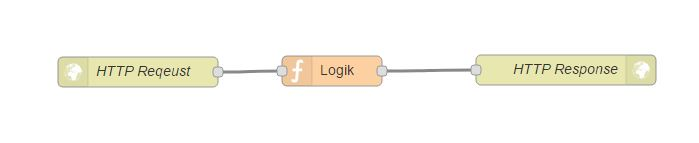
\includegraphics[scale=0.8]{images/bspFlow}
	\caption{Beispiel eines Node-RED Flows}
	\label{img:bspFlow}
\end{figure}




\section{Datenbank}%Dominic
Durch die Anbindung von Sensoren werden ständig neue Daten generiert. Damit diese Daten für spätere Zwecke genutzt werden können, wie beispielsweise für die Analyse oder Erzeugen von Vorhersagen, ist es hilfreich diese zentral an einem Ort in einer Datenbanklösung abzuspeichern.
\\NoSQL Datenbanken benötigen kein vordefiniertes Schema, um Daten abzuspeichern. Somit ist es nicht notwendig zu wissen welche Art von Daten bzw. deren Datentypen gespeichert werden sollen. Der Vorteil ergibt sich dabei, dass zusammengehörende Daten gemeinsam an einem Ort abgespeichert werden. Der Datentyp jedes einzelnen Eintrags kann dabei von Eintrag zu Eintrag variieren. Deshalb sind für diese Datenbanklösungen Strukturänderungen im Datenformat keinerlei Probleme. Sollte die Datenbank sehr groß werden und auf mehreren Servern laufen, so lassen sich diese einfach skalieren\cite{noSQL:noSQL}.
\\Außerdem gibt es noch die Möglichkeit Daten innerhalb von relationalen Datenbanken abzuspeichern. Dabei muss zuerst ein Datenbankschema definiert werden. Hierbei ist also die abzuspeichernde Datenstruktur im Voraus bereits definiert und kann im Vergleich zu NoSQL-Datenbanken nicht einfach im Betrieb angepasst werden. Die Ablagestruktur in Tabellen sollte sich dabei am natürliche Vorkommen der Daten (Bsp.: Name, Vorname, Straße, PLZ, Ort)  orientieren. Jede Zeile einer Relation steht für ein Tupel, das eine strikte Ordnung der Attribute voraussetzt\cite{codd:Codd}. Beim Einfügen muss deshalb auf die Struktur geachtet werden.
\\Da angenommen werden kann, dass die angeschlossenen Sensoren durchgängig gleiche Datenformate an den Raspberry Pi übermitteln und sich somit die Struktur nicht ändert, wird für den folgenden Verlauf der Arbeit ein relationales Datenmodell als Grundlage definiert.


Basierend auf den Grundlagen soll eine relationale Datenbank zum Speichern der Sensorwerte genutzt werden. Dabei muss die Datenbank kompatibel mit dem Raspberry Pi sein, sowie möglichst ressourcenschonend agieren. \\Es ist nicht notwendig Daten über das Netzwerk in die Tabelle einzutragen, da alle Sensoren über den Raspberry eingelesen werden können und die Datenbank somit nur lokal verfügbar sein muss.
\\Anforderungen:\\
-Lokal \\
-Schreibzugriffe über das Netzwerk\\
-Concurrent writers?\\
-Big Data -> wir haben nur kleine Datenmengen\\
-Embedded\\
-Small / Hardwareressourcen/ leichtgewichtig\\
-Portabilität\\
-User Management -> nicht notwendig\\
-Kompatibilität mit Raspberry\\

Daten nur speichern und nach außen verfügbar machen.

Vergleich in Datei schreiben, MySQL, SQLite\\
.
\subsubsection{SQLite}
Die SQLite Datenbank bietet für unsere definierten Einsatzzweck ausreichende Funktionalität an. Die Anwendung ist leichtgewichtig und läuft lokal. Außerdem verfolgt die Datenbank bei Transaktionen das ACID (atomic, consistent, isolated, durable) Prinzip. Datenbankzugriffe geschehen mit SQL. Alle Datenbanktabellen sind lokal in einer Datenbank-Datei gespeichert. Dies kann somit einfach kopiert werden, falls ein neuer Raspberry zum Einsatz kommen sollte.\\
Da jeder Raspberry seine eigene Datenbank besitzen sollte, damit keine privaten Daten zentral auf einer Datenbank abgelegt werden eignet sich SQLite ebenfalls gut.   https://www.sqlite.org/features.html
DATENTYPEN? TEXT, INTEGER, REAL, BLOB, NUMERIC, BOOLEAN, DATETIME 


\section{Regelbasiertes System} \chapterauthor{Louisa Pabst}
Im heutigen Alltag werden kontinuierlich Daten erfasst, um auf dessen Basis Informationen zu erhalten. Daten werden aus unterschiedlichen Gründen gesammelt, meist steht jedoch hinter der Datensammlung der Wunsch einen Mehrwert aus den Daten zu schaffen. Um Daten nutzen zu können, müssen diese kanalisiert, strukturiert und archiviert werden \cite{managermagazin:datensammlung}. Regelbasierte Systeme \acs{RBS}, die eine Sonderform eines Expertensystems bilden \cite{ieee:ruleBasedSystemAndNetworks}, werden für die Datenstrukturierung eingesetzt. Ursrprünglich stellten diese Systeme ledigliche mithilfe von menschlichem Expertenwissen codierte Problemlösungen dar \cite{Hayes-Roth:1985:RS:4284.4286}. Im Laufe der Zeit hat sich diese Definition erweitert. Neben Regeln, die von einem Experten gesetzt werden, stellen regelbasierte Systeme auch Regeln auf, die auf Basis historischer Datensätze erstellt werden. Aus diesem Grund wird bei der Erstellung eines solchen Systems zwischen einem experten- und einem datenbasierten Design unterschieden. Gerade im Zuge der stark ansteigenden Datenmengen findet man regelbasierte Systeme mit einem Daten basiertem Design vergleichsweise häufiger im Einsatz \cite{ieee:ruleBasedSystemAndNetworks}.\\
Die problemlösenden Methoden werden in einem \ac{RBS} durch Situation-Aktion Regeln abgebildet. Um sinnvolle Lösungen zu Problemstellungen zu erlangen, sollten die folgenden fünf Punkte beim Aufstellen von Regeln beachtet werden.\\
Das Wissen sollte in Wenn-Dann-Regeln aufgestellt werden. Die Bedingung für die Ausführung der Regel wird im ersten Teil der Regel definiert, dem Wenn-Teil. Dabei können mehrere Konditionen aneinander geknüpft werden. Im zweiten Teil der Regel, dem Dann-Teil, wird die Aktion beschrieben, die nach der Erfüllung der Kondition ausgeführt wird. Es kann davon ausgegangen werden, dass wenn die Kondition erfüllt ist, auch die Aktion erfüllt ist. Eine \ac{RBS} kann aus diesem Grund als Interpreter von Wenn-Dann-Regeln gesehen werden\cite{oracle:JREAPI}.\\
Neben der Darstellung einer Regel durch die Wenn-Dann Form, können Regeln auch durch Entscheidungstabellen abgebildet werden \cite{HSAugsburg:RuleEngine}. Entscheidungstabellen verknüpfen Aktionen mit Bedingungen \cite{itwissen:entscheidungstabelle}. Der Unterschied zu den zuvor beschriebenen Wenn-Dann-Regeln ist die formale Aufstellung der Regeln in Form von einer Tabellenstruktur.\\
Als nächsten Punkt, den man beim Aufstellen von Regeln beachten soll, ist die Steigerung der Kompetenz des \ac{RBS} proportional zur Wissenserweiterung. Wenn diese Steigerungen nicht proportional zueinander verlaufen, wird das \ac{RBS} auf lange Sicht nicht den gewünschten Mehrwert mit sich bringen.\\
Des Weiteren sollte das \ac{RBS} durch Kombination von Regeln auch komplexere Problemstellungen lösen. Dabei werden die Ergebnisse der Regelausführung sinnvoll kombiniert. Um Probleme bestmöglich lösen zu können, sollten \ac{RBS} die optimale Reihenfolge von Regeln bestimmen und anschließend ausführen. Die nach Durchführung der Regel erhaltene Lösung zur Problemstellung sollte vom System anschließend in natürliche Sprache oder in Aktionen, die für den Menschen verständlich sind, übersetzt werden.\\
Genutztes Wissen innerhalb eines \ac{RBS} wird als problemlösendes Wissen bezeichnet und besteht aus verschiedenen Formen von Informationen. So können Informationen durch Beobachtungen gesammelt werden, sowie durch Abstrahierung, Generalisierung oder Kategorisierung von gegebenen Daten. Neben reinen Daten werden Verknüpfungen von Daten sowie Stratgien zur Datengewinnung als relevante Informationen angesehen \cite{Hayes-Roth:1985:RS:4284.4286}.\\
Bei der Erstellung eines \ac{RBS} muss jedoch beachtet werden, dass ein geeignetes System stetig angepasst und verbessert werden muss. Vor allem müssen Lösungen durch hinzukommendes Wissen optimiert werden können.\cite{Hayes-Roth:1985:RS:4284.4286}.




	\chapter{Umsetzung} \label{sec:Umsetzung}
Im folgenden Kapitel wird die Umsetzung beschrieben.

\section{Datenbankschema}\label{db:DB}\chapterauthor{Dominic Steinhauser}
Innerhalb der SQLite Datenbank werden die Tabellen DHT, MQ135, Security und Window angelegt. Dadurch können die Sensordaten strukturiert in Tabellen gespeichert und die Werte mithilfe von \acf{SQL} leicht abgefragt werden. Die vier Tabellen sind auf die Anforderungen F-10.1, F-10.2, F-10.3 und F-10.4 zurückzuführen, sodass jeder Sensor seine Werte in eine eigens dafür angelegte Datenbank schreibt. Der Vorteil davon ist, dass die Übersichtlichkeit der von einem Sensor erzeugten Daten gewährleistet ist.\\
Jede Tabelle besitzt pro Relation eine eindeutige ID. Dies hilft einen Datensatz eindeutig zu identifizieren. Neben der ID kann der Timestamp ebenfalls als eindeutige Identifizierung eines Datensatzes genutzt werden, da es sehr unwahrscheinlich ist, dass innerhalb einer Millisekunde zwei Datenbankeinträge in einer Tabelle erstellt werden.\\

Daten aus dem DHT22 Sensor (Temperatur- \& Luftfeuchte) werden in der Tabelle DHT in den folgenden Spalten abgespeichert:
\begin{itemize}
	\item \textbf{ID}: Primärschlüssel, der nicht leer sein darf und sich inkrementell erhöht.  
	\item \textbf{Temperature}: Temperaturwert in Celsius wird als REAL Number gespeichert.
	\item \textbf{Humidity}: Prozentwert der Luftfeutchtigkeit wird als REAL Number gespeichert.
	\item \textbf{Sensorid}: Text, der angibt um welche Art von Temperatur- \& Luftfeuchtigkeitssensor es sich handelt.
	\item \textbf{Timestamp}: Zeitstempel wird in Millisekunden als Integer gespeichert
\end{itemize}

Die Window Tabelle nimmt die Werte des Magnetkontakts entgegen und speichert diese:
\begin{itemize}
	\item \textbf{ID}: Primärschlüssel, der nicht leer sein darf und sich inkrementell erhöht.  
	\item \textbf{Value}: Integer, entweder 1 für geöffnetes Fenster oder 0 für geschlossen.
	\item \textbf{Timestamp}: Zeitstempel wird in Millisekunden als Integer gespeichert
	\item \textbf{Room}: Beschreibung, in welchem Raum der Fensterstatus geprüft wird. 
\end{itemize}

Der MQ-135 Sensor speichert die verschiedenen Werte der Gase CO2, CO und NH4 in folgenden Spalten ab.
\begin{itemize}
	\item \textbf{ID}: Primärschlüssel, der nicht leer sein darf und sich inkrementell erhöht.  
	\item \textbf{CO2}: CO2 Wert in parts per million (ppm) wird als REAL abgespeichert.
	\item \textbf{CO}: CO Wert (ppm) wird als REAL abgespeichert.
	\item \textbf{NH4}: NH4 Wert (ppm) wird als REAL abgespeichert. 
	\item \textbf{Timestamp}: Zeitstempel wird in Millisekunden als Integer gespeichert
\end{itemize}

Sobald die Bibliothek Motion eine Bewegung erkennt, wird automatisch ein Datenbankeintrag generiert der die nachfolgende Struktur aufweist:
\begin{itemize}
	\item \textbf{ID}: Primärschlüssel, der nicht leer sein darf und sich inkrementell erhöht.  
	\item \textbf{Camera}: Integer, der angibt welche Kamera das Bild aufgenommen hat.
	\item \textbf{Filename}: Text, der angibt unter welchem Pfad das Bild gefunden werden kann.
	\item \textbf{Frame}: Integer, der angibt welches aus dem Video extrahiert wurde. 
	\item \textbf{File\_type}: Integer, der angibt um was für eine Datei es sich handelt.
	\item \textbf{Timestamp}: Zeitstempel, der als im Format \enquote{YYYY-MM-DD HH:MM:SS} angibt, wann die erste Bewegung erkannt wurde.	
\end{itemize}


\section{Raspberry Pi} \chapterauthor{Dominic Steinhauser}
Im folgenden Abschnitt wird beschrieben, wie der Raspberry Pi mit den Sensoren interagiert, die Daten speichert und anschließend über Services bereitstellt.

\subsection{Sensor Adapter - Datenbeschaffung}
Der Raspberry Pi bildet die zentrale Einheit, um verschiedene Sensoren in eine Anwendung zu integrieren. Dabei spielen dessen externe Schnittstellen eine wesentliche Rolle. Allerdings liegt der Fokus dieser Arbeit auf der Datenbereitstellung über einen Webserver, dem Verarbeiten und Anzeigen in der App, weshalb teilweise auf bereits bestehende Lösungen zurückgegriffen wird.
\\\\Das \acf{CSI} stellt eine Möglichkeit dar, eine eigens für den Raspberry Pi entworfene Kamera anzuschließen. Das Kameramodul kann dann über entsprechende Befehle über die Kommandozeile des Raspberry Pis gesteuert werden. Aus der Anforderung F-10.1 geht hervor, dass Bilder bei erkannter Bewegung gespeichert und einen Livestream umgesetzt werden sollen.\\Die Anzeige eines Live-Bildes könnte über eine sekündliche Aufnahme, die über eine Service unter einer Internetadresse verfügbar gemacht wird, umgesetzt werden. Ob innerhalb eines Bildes Bewegung erkannt wird, könnte durch eine Vergleich eines Referenzbildes und dem aktuellen Bild ermittelt werden.\\Allerdings bietet diese Funktionalitäten bereits das Open-Source Programm \enquote{Motion} an. Es ist in der Lage Bewegung zu erkennen, Live-Bilder anzuzeigen und erkannte Bewegung in Form von Events abzuspeichern.\cite{motion:Motion}\\
\\Motion wurde so konfiguriert, dass der Livestream über die \ac{IP}-Adresse des Raspberry Pis und dem Port 8081 erreichbar ist. Eine Bewegung wird erkannt, wenn sich drei aufeinanderfolgenden Bilder um 15000 Pixel zum Referenzbild unterscheiden. Dabei ist eine Auflösung von 640x480 Pixel gewählt. Wenn für sieben Sekunden keine Bewegung mehr wahrgenommen wird, ist das Event beendet. Für jedes Event wird in der Tabelle Security (siehe \autoref{db:DB}) ein Datenbankeintrag erstellt. Außerdem wird ein Video in einem definierten Verzeichnis abgespeichert, das die ganze Sequenz der Bewegungserkennung enthält. Nachdem das Video erstellt wurde, wird außerdem noch ein Bild extrahiert, das anzeigt wer die Bewegung ausgelöst hat. Dadurch erhält der Anwender frühzeitig Klarheit, wer sich im Raum befindet.
\\\\
Die Sensoren für Luftfeuchtigkeits- bzw. Temperaturmessung, den Magnetkontakt für die Prüfung, ob ein Fenster offen oder geschlossen ist, sowie den Luftqualitätssensor werden über die Pins des \ac{GPIO} angeschlossen. Im Gegensatz zum MQ-135 Sensor liefern der DHT22 Sensor (Temperatur \& Luftfeuchte) und der Magnetsensor digitale Werte zurück. Die digitalen Werte können mithilfe der \enquote{bcm2835}-Bibliothek \ac{GPIO} ausgelesen werden\cite{bcm:Bcm}. Die Knoten \enquote{Node-Red-Contrib-Gpio}\cite{node:GPIO} und\enquote{Node-red-contrib-dht-sensor}\cite{node:DHT22} werden dazu genutzt, um die Werte des Magnet- bzw. DHT22 Sensors in Node-Red zur Verfügung zu stellen. 
\\
\autoref{flow:tempDB} zeigt den simplen Flow, damit alle 5 Minuten der aktuelle Sensorwert in die Tabelle DHT eingetragen wird. Dazu ist es notwendig einen Input Node zu verwenden und so zu konfigurieren, dass alle 5 Minuten ein Event ausgelöst wird. Wenn ein Event beim DHT Sensor ankommt (2. Node), reicht über eine Nachricht die aktuellen Temperatur- und Luftfeuchtigkeitswerte weiter an den Funktionsknoten.
\begin{figure}[h]
	\centering
	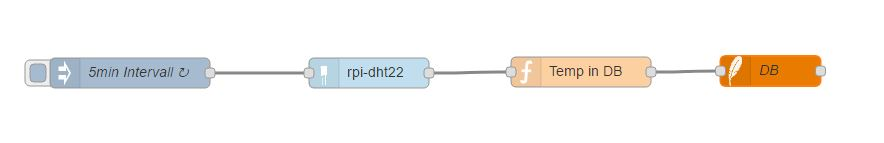
\includegraphics[scale=0.7]{images/tempIntoDB}
	\caption{Temperatur/ Luftfeuchtigkeit in Datenbank}
	\label{flow:tempDB}
\end{figure}
\\\autoref{list:tempIntoDB} zeigt, wie im Funktionsknoten die aktuellen Werte des DHT Sensors aus dem \enquote{msg} Objekt ausgelesen und dem neu erstellen \ac{JSON}-Objekt \enquote{newMsg} im \ac{SQL} Statement übergeben werden. \\Der SQLite Node nimmt anschließend das Event und die neu angelegte Nachricht entgegen und führt den \ac{SQL} Befehl  aus. Dazu muss der \ac{SQL} Befehl immer im zu übergebenen Objekt unter dem Schlüssel \enquote{topic} abgelegt sein. Auffallend hierbei ist, dass anstatt einer ID \enquote{NULL} übergeben wird. Da die Spalte ID Primarschlüssel ist und nicht leer sein darf, wird von SQLite automatisch die neue ID gesetzt.
\begin{lstlisting}[label=list:tempIntoDB, caption={Neuer Eintrag in Tabelle DHT}]
var date = Date.now();
var newMsg = {
"topic": "INSERT INTO DHT VALUES(NULL,"+msg.payload+","+msg.humidity+ ", '"+msg.sensorid+"', "+date+")"
}
return newMsg;
\end{lstlisting}
Der Datenfluss für das Eintragen des Status, ob das Fenster geöffnet oder geschlossen ist (vgl. \autoref{flow:winDB}), hat einen ähnlichen Aufbau wie der Datenfluss in \autoref{flwo:tempDB}. Der Konten \enquote{Pin: 18} sendet immer nur dann ein Event aus, sobald sich eine Zustandsänderung gibt. Damit Rückschlüsse auf die Daten verschiedener Sensoren besser getätigt werden können, speichert der \enquote{Inject}-Node ebefalls im Intervall von 5 Minuten den aktuellen Zustand ab. 
Außerdem stützen mehrere Werte die Genauigkeit von Vorhersagen und Analysen lassen sich leichter generieren, indem in verschiedenen Tabellen nach dem gleichen Zeitstempel gesucht wird.
\begin{figure}[h]
	\centering
	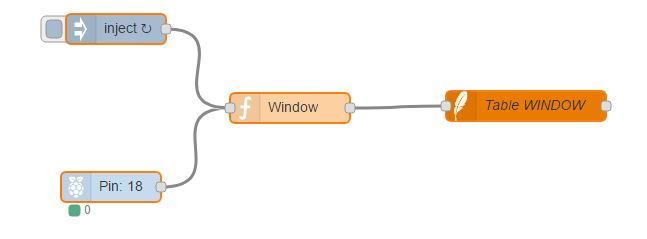
\includegraphics[scale=0.7]{images/windowIntoDB}
	\caption{Fensterstatus in Datenbank}
	\label{flow:winDB}
\end{figure}

Der MQ-135 Sensor gibt ein analoges Signal zurück, das in ein digitales Signal umgewandelt werden muss, damit der Raspberry dieses verarbeiten kann. Es ist also erforderlich, dass ein Analog-Digital-Wandler das Ausgangssignal des Sensors in ein für den Raspberry verständliches digitales Signal umwandelt. Dazu kann der MCP3008 Analog-Digital-Wandler verwendet werden. Da Node-RED hierfür keine Lösung anbietet, werden über Python die Datenbankeinträge für den Sensor erstellt.
\\Eingehende Signale können dann über den \acf{SPI} Bus ausgelesen werden. Der MCP3008 liefert Werte zwischen 0 und 1023 (10Bit) an den Raspberry Pi weiter. Um aus den Werten die Spannung und daraus dann die Gaskonzentration ableiten zu können, ist folgende Formel zu beachten\cite{gas:MQX}:\\
\begin{center} Ausgangsspannung $=  \frac{ADC Wert}{1023} *  $ angelegte Spannung\end{center}

Damit nun die tatsächlichen Gaswerte ermittelt werden können, muss zuerst eine Kalibrierung des Sensors erfolgen. In dieser Phase geht der Sensor davon aus, dass er sich in reiner, guter Luft befindet. Ausgehend von der Kalibrierung gleicht der Sensor dann die ankommenden Daten mit einer speziell für eine Gaswert definierten Geraden ab. Dafür muss aus den Charakteristiken jedes Gases \footnote{Seite 2, https://www.olimex.com/Products/Components/Sensors/SNS-MQ135/resources/SNS-MQ135.pdf} eine entsprechende Geradengleichung ermittelt werden. Die ankommenden Daten eines Gases werden dann mit der entsprechend definierten Geraden des Gases verglichen und die Gaskonzentration ausgegeben.\cite{gas:MQ}. Der Quellcode für die Auswertung der Eingangswerte ist in \autoref{list:MQClass} aufgezeigt.
\\ \autoref{list:MQGas} zeigt den Quellcode auf, der die berechneten Gaswerte in die Datenbank schreibt. Damit Ausreißer nicht ins Gewicht fallen, werden 15 Gaswerte in einem Array gespeichert, sortiert und der Median abgespeichert. Die Generierung eines neuen Datenbankeintrags wird dabei in Zeile 13 dargestellt. In die Datenbank eingefügt wird ein Zeitstempel in Millisekunden, sowie die Werte der verschiedenen Gase.

\begin{lstlisting}[label=list:MQGas, caption={MQ-135 Sensorwerte in DB}]
while True:
	temp = [[], [], []]
	n = 15
	for i in range(n):
		perc = mq.MQPercentage()
		temp[0] += [perc["CO2"]]
		temp[1] += [perc["CO"]]
		temp[2] += [perc["NH4"]]
		time.sleep(2)
	temp[0] = sorted(temp[0])
	temp[1] = sorted(temp[1])
	temp[2] = sorted(temp[2])
	c.execute("INSERT INTO mq135(timestamp, CO2, CO, NH4) VALUES(?, ?, ?, ?)",(int(time.time()*1000), temp[0][int(math.floor((n-1)/2))], temp[1][int(math.floor((n-1)/2))], temp[2][int(math.floor((n-1)/2))]))
conn.commit()
\end{lstlisting}


\subsection{Services Node-RED}
Damit die gespeicherten Daten zu den verschiedenen Sensoren auch für andere Anwendungen bereitgestellt werden können, werden mithilfe des Node-RED-Webservers REST Servies angelegt. Diese können über \ac{HTTP} Anfragen angesprochen werden und liefern als Ergebnis Daten im \ac{JSON}-Format zurück. Dabei wird je nach angesprochenem Pfad ein bestimmtes Ergebnis zurückgeliefert. \\Anfragen müssen an den Raspberry Pi bzw. dessen Webserver-Schnittstelle gesendet werden. Dabei ist darauf zu achten, dass sich der Node-RED-Webserver unter der \ac{IP}-Adresse des Raspberry Pis und dem Port 1880 erreichen lässt. Als Beispiel könnte die Adresse folgendes Format haben: 192.168.0.100:1880. \\Damit nun ein entsprechender Service aufgerufen wird, muss noch eine Pfad an die \ac{URL} angehängt werden. In Node-Red wurden folgende REST \ac{API} Schnittstellen entwickelt:
\begin{itemize}
	\item \textbf{/temp}: Diese Route liefert dem Anwender den aktuell gemessenen Wert vom Temperatur- \& Luftfeuchtigkeitssensor  zurück. 
	\item \textbf{/tempInt}: Um sich den Temperaturverlauf innerhalb eines begrenzten Zeitraums anzeigen zu lassen, kann diese Route angesprochen werden. Dabei müssen ein Startdatum, sowie ein Enddatum jeweils im Format \enquote{dd.mm.yyyy} als Parameter der Anfrage mit übergeben werden.
	\item \textbf{/window}: Gibt den aktuellen Status zurück, ob das Fenster geöffnet oder geschlossen ist.
	\item \textbf{/motion}: Liefert als Ergebnis eine ID und einen Zeitstempel zurück, um dem Anwender mitzuteilen zu welchem Zeitpunkt eine Bewegung erkannt wurde.
	\item \textbf{/picture}: Dieser Service benötigt als Parameter eine ID, die über den Pfad \enquote{/motion} ermittelt werden kann. Durch diese ID kann dann der Pfad zum entsprechenden Bild geladen werden und als Antwort wird das Bild dem Anwender angezeigt.
	\item \textbf{/mqgas}: Die aktuellen Gas-Werte können über den Service herausgefunden werden.
	\item \textbf{/gasInt}: Gleiches Prinzip, wie bei der Route \enquote{/tempInt}. Dem Request werden zwei Parameter (Startdatum, Enddatum) übergeben und die Gaswerte zurückgeliefert, die im angegebenen Zeitraum erfasst wurden.
\end{itemize}

\autoref{flow:TempInt} stellt beispielhaft den Node-RED-Flow zum Abfragen des Temperatur- und Luftfeuchtigkeitsverlaufs dar. Der Service wird angesprochen, wenn folgender Pfad adressiert wird: /tempInt?from=10.05.2017\&to=22.05.2017. Mit dieser Anfrage werden alle gespeicherten Werte als Antwort zurückgeliefert, die im entsprechenden Intervall liegen.
\begin{figure}[h]
	\centering
	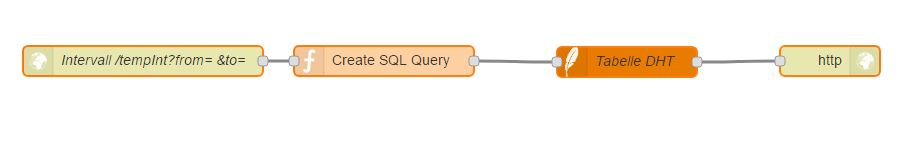
\includegraphics[scale=0.7]{images/tempIntFlow}
	\caption{Beispiel: Temperatur Intervall abfragen}
	\label{flow:TempInt}
\end{figure}
Der erste Node wird dazu benötigt, um eine HTTP Request anzunehmen. Dabei ist die Route zu definieren, unter der der Service erreichbar sein soll. In diese Fall ist dies \enquote{/tempInt}. Die übergebenen Parameter werden erst im Funktionsknoten betrachtet, d. h. die eingehenden Parameter werden über ein JSON-Objekt an den nachfolgenden Knoten übergeben. 
\\\autoref{list:tempInt} ist der Quellcode des Funktionsknotens. In Zeile 3 wird geprüft, ob beide Parameter gesetzt sind. Falls dies nicht der Fall ist, sollen die letzten 20 Einträge aus der Datenbank geladen werden (siehe Zeile 24 \autoref{list:tempInt}). Dieser Schritt ist notwendig, da der nachfolgende Knoten auf die Datenbank zugreift. Liegt keine Abfrage vor, so wird ein Fehler zurückgeworfen und der Flow  unterbrochen. 
\\Falls beide Parameter gesetzt wurden, müssen JavaScript Zeitstempel generiert werden, da nur solche in der Datenbanktabelle DHT gespeichert sind. Hierfür werden in Zeile 10f die beiden Strings in Arrays unterteilt, sodass das Jahr, der Monat und die Tage separiert sind. Anschließend kann mithilfe des Date Objektes ein Zeitstempel generiert werden. Dabei ist darauf zu achten, dass JavaScript in den Monaten bei \enquote{0} zu zählen beginnt und somit der Monat um eins reduziert werden muss. \\Der timestampTo wird außerdem noch mit 23 Stunden, 59 Minuten und 59 Sekunden erzeugt, damit ein einzelner Tag auch respektiert werden kann. \\Sobald beide Zeitstempel vorliegen, wird die \ac{SQL} Abfrage generiert und in der Variable \enquote{selectString} gespeichert. \\Zum Schluss muss die Abfrage in einem JavaScript Objekt als Key-Value übergeben werden. Die Datenbankabfragen müssen dabei immer unter dem Key \enquote{topic} abgelegt sein. Zum Schluss wird das Objekt dann noch zurückgegeben, sodass es vom nächsten Node verwendet werden kann. 
\begin{lstlisting}[label=list:tempInt, caption={Funktion Node-RED tempInt}]
var selectString;

if(msg.req.query.from && msg.req.query.to){
	var fromDate = msg.req.query.from;
	var toDate = msg.req.query.to;
	
	/*convert date into timestamp
	first divide date string into day, month, year 
	then create new Date to get an timestamp*/
	var fDate = fromDate.split("."); 
	var tDate = toDate.split(".");
	
	/*create timestamp; month-1 because Jan = 0, Feb = 1 etc.
	date requires the order: year, month, day, hours, minutes, seconds */
	var timestampFrom = new Date(fDate[2], fDate[1]-1, fDate[0]).getTime();
	//to respect the whole day set hours, minutes, and seconds
	var timestampTo = new Date(tDate[2],tDate[1]-1, tDate[0], 23, 59, 59).getTime();
	
	var select = "Select * FROM DHT WHERE timestamp >= "; 
	var and = " AND timestamp <=";
	selectString =select + timestampFrom + and + timestampTo;
}
else {
	selectString = "Select * FROM DHT ORDER BY ID DESC LIMIT 20";
}

//create Message object for db access
var newMsg = {};
newMsg.topic = String(selectString);
return newMsg;
\end{lstlisting}

Nachdem die Abfrage im entsprechenden Objekt vorliegt, kann der Datenbankknoten die Anfrage verarbeiten und die ermittelten Ergebnisse werden an die \ac{HTTP} Node gesendet. Dabei muss in dem SQLite Node der Pfad zur SQLite Datenbank gesetzt werden.
\\\autoref{list:temp}  zeigt das \ac{JSON}, das vom Webserver als Antwort zurückgeliefert wird. Dieses hat durchgehend die gleiche Struktur und kann somit nach dem Key-Value-Prinzip ausgelesen werden. Enthält eine Antwort mehrere Einträge, wird ein Array mit mehreren Objekten zurückgeliefert.
\begin{lstlisting}[label=list:temp, caption={Beispiel: JSON Response für den Pfad: /temp}]
{
	"temp": "24.60",
	"humidity": "46.60",
	"sensorid": "dht22",
	"date": 1495920298490
}
\end{lstlisting}


\section{Mobile Android Applikation}
Als grafische Benutzerschnittstelle , für das in dieser Arbeit erläuterte System, wird eine ortsunabhängige Lösung entwickelt (F-10.2). Um eine Ortsunabhängigkeit gewährleisten zu können, bietet es sich an, ein mobiles Endgerät zu entwickeln. Es wurde  entschieden als Benutzerschnittstelle eine Android App zu nutzen, da das Android-Betriebssystem den höchsten Endkundenabsatz besitzt \cite{statista:marktanteileandroid} und dadurch eine größere Masse erreicht werden kann.

\subsection{Architektur der mobilen Android Applikation}\chapterauthor{Louisa Pabst}
Auf Grundlage der Anforderungen wird die Architektur der mobilen Android Applikation erstellt.
In der Architektur werden alle wichtigen Entscheidungen, welche für die Entwicklung des Systems relevant und von technischer Natur sind, berücksichtigt. Die Architektur dient als Grundlage für die darauffolgende Umsetzung der Applikation.\\
Um die Anwendung strukturierter entwickeln zu können, wird ein Entwurfsmuster zur Strkturierung der Applikation genutzt. Als Entwurfsmuster bietet sich das \ac{MVC} Entwurfsmuster an. Das \ac{MVC} Designpattern beschreibt eine Architektur zum Anordnen von Objekten. Das \ac{MVC} Entwurfsmuster ermöglicht dabei, einen großen Spielraum für individuelle Anpassungen, weil es nicht starr definiert ist \cite{bucanek:modelviewcontroller}.\\
MVC ermöglicht zwischen der Anzeige der Daten, der Datenverwaltung und der Datenspeicherung eine Unabhängigkeit der Daten zu gewährleisten. So müssen bei Veränderungen des Datenmodells keine Anpassungen an der grafischen Benutzerschnittstelle direkt durchgeführt werden. Es können auch mehrere Views zu einem Model gehören ohne sich gegenseitig zu behindern. Was beachtet werden muss, ist das ein \ac{MVC} Entwurfsmuster bei kleinen Softwareprojekten schnell den Code unnötig aufblasen lässt. Innerhalb dieser Arbeit wird es jedoch als sinnvoll erachtete und genutzt. Zum einen das komplexe Datenmodell und zum Anderen die visuelle Aufbereitung der Daten rechtfertigen die Nutzung eines MVC Musters. Eine Wartung des Quelltextes wird durch ein \ac{MVC} Entwurfsmuster erleichtert, da es hilft den Code übersichtlich aufzuteilen \cite{bucanek:modelviewcontroller}.


\subsection{Rule Engine}\chapterauthor{Louisa Pabst}
Vor Beginn der Entwicklung muss die Struktur von Regeln analysiert werden. Eine Regel besteht aus einem Wenn-Teil und dem Dann-Teil. Der Wenn-Teil wiederum kann aus mehreren einzelnen Wenn-Teile zu einem übergreifenden Wenn-Teil zusammengefasst werden. Das Zusammenfassen mehrerer Wenn-Teilen führt zu mehr Regelmöglichkeiten. Der gleiche Grund kommt bei dem Dann-Teil zum Tragen. Gerade im Hinblick auf die Integration von weiteren Akteuren (F-60.2) ist es sinnvoll, mehrere Akteure innerhalb einer Regel auslösen zu können.\\
Ein einzelner Wenn-Teil der Regel besteht aus einem Datentypen, Vergleichsoperator/en, Vergleichsdaten und einer Konjunktion zu einem anderen Wenn-Teil. Um dem Nutzer eine intuitivere Anwendung bieten zu können, werden Vergleichsoperatoren in Regeln angeboten, die aus zwei Operatoren bestehen. So können Vergleichsoperatoren, wie ``zwischen'' gewährleistet werden. Ein Wert ist dann zwischen zwei Werten, wenn der Datenwert größer als Vergleichswert 1 und kleiner als Vergleichswert 2 ist. Innerhalb der Rule Engine wird dementsprechend zwischen klassischen binären und zusammengesetzten binären Operatoren unterschieden. Binäre Operatoren vergleichen zwei Werte miteinander \cite{unilinz:binaereoperatoren}.\\
Erstellte Regeln werden dem Ersteller direkt zugeordnet. Die Sensordaten sind im Gegensatz nicht Nutzern zugeordnet, sondern einem Raspberry Pi. Das bedeutet mehrere Bewohner eines Hauses können auf die gleichen Sensoren zugreifen, sich aber individuelle Regeln auf ihre Bedürnisse hin definieren.\\
Die Rule Engine wird nach den Anforderungen aus Kapitel \ref{sec:Anforderungen} entwickelt. Demnach muss die Rule Engine dem Nutzer ermöglichen, dynamisch Regeln hinzufügen oder wieder zu löschen zu können. (F-30.1). Grenzwerte oder Wertebereiche kann der Nutzer für die erfassten Datentypen (F-10) selbst bestimmen (F-30.2). Des Weiteren soll die Rule Engine zeitliche Aspekte in den Regeldefinitionen einbinden können. Der Nutzer kann demnach zeitliche Intervalle festlegen, in denen ein Wert oder Wertebereich gehalten werden soll. Die Definition von Datenabhängikeiten kann von der Rule Engine verarbeitet werden, um optimalere Aktionen auslösen zu können (F-30.5).\\
Es werden mögliche Rule Engines recherchiert, die die gestellten Anforderungen erfüllen. Dabei wurden nur Rule Engines betrachtet, die in Android genutzt werden können, sowie welche mit regelmäßigen Releases. Aus der Recherche haben sich folgende Rule Engine Bibliotheken ergeben:
\begin{itemize}                                                                                                               
	\item Easy Rules \cite{github:easyrules}
	\item OpenRules \cite{openrules}
	\item RuleBook \cite{github:rulebook}
\end{itemize}
Diese Rule Engines bieten gute Möglichkeiten Regeln zu erstellen und diese zu überprüfen. Regeln für bestimmte Werte können zur Laufzeit hinzugefügt werden. Dies ist im Hinblick auf die Sensorenerweiterung durchaus sinnvoll. Jede Regel muss jedoch hartcodiert vor der Laufzeit in die Rule Engine hinzugefügt werden. Das ist ein entscheidener Nachteil dieser Rule Engines. Durch die Recherche konnte keine Engine gefunden werden, die eine dynamische Erstellung von neuen Regeln über die Oberfläche ermöglicht. Die Definition neuer Regeln durch den Nutzer ohne den Quellcode zu verändern, ist jedoch eine essentielle Anforderung. Aus diesem Grund wurde sich dafür entschieden, eine Rule Engine selbst zu implementieren.\\
Bei der Implementierung der Rule Engine wurden die Ergebnisse der Recherche miteinbezogen. Vor allem die Struktur der Regeln zu ihren Wenn- und Dann-Teilen der Regel Engine RuleBook wurde bei der Implementierung betrachtet.\\
Für die Strukturierung der Rule Engine wurden mögliche Lösungswege betrachtet. Eine Möglichkeit wäre jede Regel als Java-Klasse zu erstellen. Jede spezifische Regel würde dann von der Klasse Regel erben, sodass die Haupteigenschaften in jeder Klasse erhalten sind. Um dem Nutzer das Hinzufügen einer neuen Regel zur Laufzeit zu ermöglichen,müsste eine neue spezifische Regel-Klasse zur Laufzeit hinzugefügt werden.

Das Hinzufügen von Klassen zur Laufzeit hat vor allem vier Nachteile, die in unserem Kontext relevant sind. Der erste Nachteil ist die Umgebung, in der der Quellcode ausgeführt werden muss. Zur Kompilierung zur Laufzeit muss die Umgebung eine JDK besitzen. Ohne JDK ist das Hinzufügen von Klassen zur Laufzeit nicht möglich. Ein weiterer Nachteil ist die Komplexität. Durch das Kompilieren von Klassen zur Laufzeit entsteht eine erhöhte Komplexität, aus der auch der dritte Nachteil resultiert. Die Geschwindigkeit der Applikation wird beeinträchtigt. Gerade bei einer mobilen Applikation möchte ein Nutzer nicht lange auf das Ergebnis warten. Der letzte entscheidene Nachteil ist die Sicherheit. Wenn dem Nutzer die Möglichkeit gegeben wird zur Laufzeit eine Regel hinzuzufügen, kann dieser versuchen Schadcode einzubauen. Bei erfolgreicher Schadcode-Einbettung ist die gesamte Applikation stark beeinträchtigt.\\
Eine weitere Möglichkeit eine Rule Engine zu implementieren, ist diese mit Hilfe eines JavaScript Interpreters zu realisieren. Die Regel wird dabei in JavaScript Code abgespeichert. Bei Ausführung der Rule Engine wird dann der JavaScript Code interpretiert. Auch bei dieser Möglichkeit der Umsetzung ist die Sicherheit ein entscheidender Nachteil. Es muss verhindert werden, dass der Nutzer bei der Spezifikation der Regel Schadcode einfügen kann, die dann durch den Interpreter ausgeführt wird. Um JavaScript auf einem Android Gerät ausführen zu können, muss ein leichtgewichtiger JavaScript Interpreter gefunden werden, damit die Schnelligkeit der Anwendung nicht darunter leidet. Es wurden Rhino, Nashorn und J2V8 als mögliche  JavaScript Interpreten untersucht.\\
Rhino ist eine JavaScript Engine mit der es möglich ist JavaScript in Java Bytecode zu kompilieren und zur Laufzeit zu interpretieren.\cite{mozilla:rhino}. Rhino lässt sich zudem in Android einbinden. Ein Nachteil von Rhino ist die Komplexität. Innerhalb dieser Arbeit werden nur unkomplizierte if-Abfragen mit einem String Rückgabewert in JavaScript interpretiert werden müssen. Nashorn ist ein Nachfolger des Rhino Interpreters. Nashorn kommt nicht als Interpreter innerhalb dieser Arbeit in Frage, da dieser keine Integration in Android zulässt.\\
Eine weitere Möglichkeit ist die Verwendung der J2V8 JavaScript Engine \cite{github:j2v8}. Diese Engine ist eine leichtgewichtige Form der V8 Engine. V8 ist eine Google Open Source JavaScript Engine \cite{github:v8}. Der entscheidende Vorteil von J2V8 gegenüber der V8 Engine ist die Performanceverbesserung. J2V8 eignet sich dementsprechend gut für die Integration in dieser Arbeit.\\
Um die J2V8 Engine nutzen zu können, muss eine Laufzeitumgebung erstellt werden. Zu dieser Umgebung kann anschließend JavaScript Code hinzugefügt werden, der ausgeführt wird. Dabei muss angegeben werden um welchen Rückgabewert es sich handelt. Der Rückgabewert wird dann an den Java Code übergeben. Durch die Interpretation von JavaScript kann die Rule Engine auf eine Methode reduziert werden. Im Folgenden Code ist diese aufgezeigt.
\begin{lstlisting}[language=java]
	public void run(HashMap<String, String> values){
		PushMessage push = new PushMessage();
    	V8 runtime = V8.createV8Runtime();
        List<String> rules = db.getRuleStrings(db.getloggedInUser());
        Iterator it = values.entrySet().iterator();
        while (it.hasNext()) {
            Map.Entry entry = (Map.Entry) it.next();
            variables += "var " + entry.getKey().toString() + " = " + entry.getValue() + ";";
        }
        for (int r = 0; r < rules.size(); r++) {
            String rule = rules.get(r);
            String notificationText = runtime.executeStringScript(variables + rule);
            runtime.release();
            if(!notificationText.isEmpty()) {
                push.sendNotification(notificationText);
        }
    }
\end{lstlisting}
Die Überprüfung einer Regel wird in drei Schritten durchgeführt.
\begin{enumerate}
\item Im ersten Schritt werden die Variablen der JavaScript Umgebung hinzugefügt. Die Variablen sind die Datentypen, die von den Sensoren übergeben werden. Auf die genaue Kommunikation der Daten von Node-RED zur Regel Engine wird später eingegangen. Die Regel Engine kann dabei unterschiedliche Datentypen übergeben bekommen, die nicht fest definiert sein müssen. 
\item Im zweiten Schritt wird die Regel in JavaScript Format ausgeführt. Die Regel ist eine if-Abfrage, die bei Erfüllung der Kondition einen Text ausgibt. Der Text beinhaltet den Handlungsvorschlag an den Nutzer.
\item Im dritten Schritt wird eben dieser Handlungsvorschlag an die Java Umgebung zurückgegeben, um dem Nutzer über eine Benachrichtigung den Handlungsvorschlag zu eröffnen.
\end{enumerate}

\subparagraph{Kommunikation der Sensordaten}
Im Folgenden wird näher auf die Kommunikation der Sensordaten von Node-RED an die App zur Regelkontrolle eingegangen.\\
Die Daten müssen gebündelt an die App kommuniziert werden.\\
Entweder können die Daten nach einem bestimmten Zeitintervall von der App durch einen HTTP Request eingefordert werden oder durch Node-RED die Daten in regelmäßigen Zeiteinheiten an die App gesendet werden. Es wurde sich innerhalb dieser Arbeit dafür entschieden die Nachrichten von Node-RED schicken zu lassen, damit im Hintergrund der App so wenig wie möglich von der App ausgeführt werden muss. Gerade bei mobilen Applikationen muss darauf geachtet werden, die Batterie und die Netzanbindung so gering wie möglich zu belasten. \\
Die Daten werden im JSON-Format mit Hilfe von \ac{FCM} an die App gesendet \cite{firebase:gcm}. Der zeitliche Rythmus der Datenversendung kann über das Node-RED Interface eingestellt werden. \ac{FCM} bietet drei Möglichkeiten an, das Ziel der Nachricht zu definieren.
\begin{itemize}
	\item Nutzersegment: Nachricht wird an alle geräte eines bestimmten Nutzersegmentes versendet
	\item Thema: Nachricht wird an alle Geräte gesendet, die sich zu einem Thema aboniert haben
	\item Einzelnes mobiles Gerät: Nachricht wird an ein einzelnes Gerät gesendet
\end{itemize}
Für Testzwecke wurde sich entschieden, die Nachrichten an einzelne Geräte zu versenden. Wenn ein Sensorsystem jedoch mehrere Nutzer besitzt, bietet es sich an für jedes Sensorsystem ein Thema zu erstellen, zu dem sich die Nutzer registrieren können.\\
Die Abbildung \ref{fig:sequenzdiagramm} zeigt in Form eines Sequenzdiagrammes den Verlauf von der Übermittlung
der Daten von Node-RED an die App bis zur Auslösung der Aktion an.
\begin{figure}
	\centering
	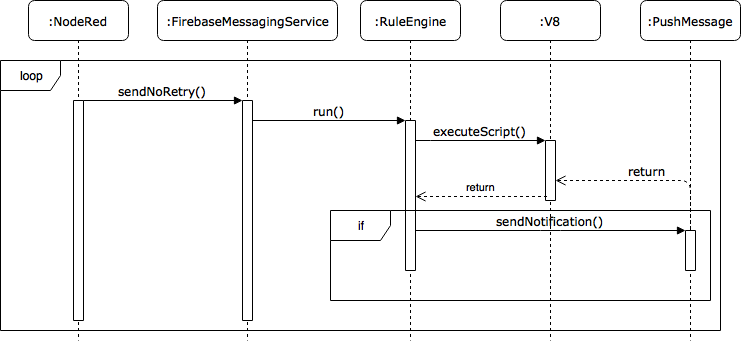
\includegraphics[width=1\textwidth]{images/Sequenzdiagramm.png}
	\caption{Sequenzdiagramm zur Regelkontrolle}
	\label{fig:sequenzdiagramm}
\end{figure}

Bei der Häufigkeit der Benachrichtigungen an den Nutzer muss darauf geachtet werden, dass nicht zu viele Nachrichten an den Benutzer geschickt werden. Bei einer zu großen Häufigkeit an Benachrichtigungen kann der Nutzer diese als eine Belästigung ansehen \cite{gadgets:amountnotifications}. Eine geeignete Anzahl an Benachrichtigungen kann als feste Zahl nicht genannt werden und sollte an den Use Case so gut wie möglich angepasst werden.

\subsection{Daten Anzeige}\chapterauthor{Dominic Steinhauser}
\autoref{label:main} zeigt die Startseite der Anwendung. Sie bietet schnellen Zugriff auf alle ausführbaren Aktionen in der App.
\\Beim Aufrufen der \enquote{AirQuality}-View wird eine \ac{HTTP} Anfrage an den Webserver gesendet. Die zurückgelieferten Ergebnisse, welche den aktuell gemessenen Sensorwerten entsprechen, werden in \autoref{label:airquality} neben ihrer Beschreibung dynamisch gesetzt und liefern so dem Anwender erste Informationen zu seiner Umgebung. Da allerdings nur die aktuellen Sensorwerte in dieser Ansicht angezeigt werden, kann der Anwender über den Pfeil zur nächsten Seite navigieren, die es dann ermöglicht den Verlauf der Daten anzuzeigen. Aus einem Diagramm lassen sich die Werte schnell und einfach ablesen. Außerdem zeigt ein Verlauf, wie sich die Daten im Verhältnis zur Zeit entwickelt haben.

\begin{minipage}[c]{0.5\textwidth}
	\centering
	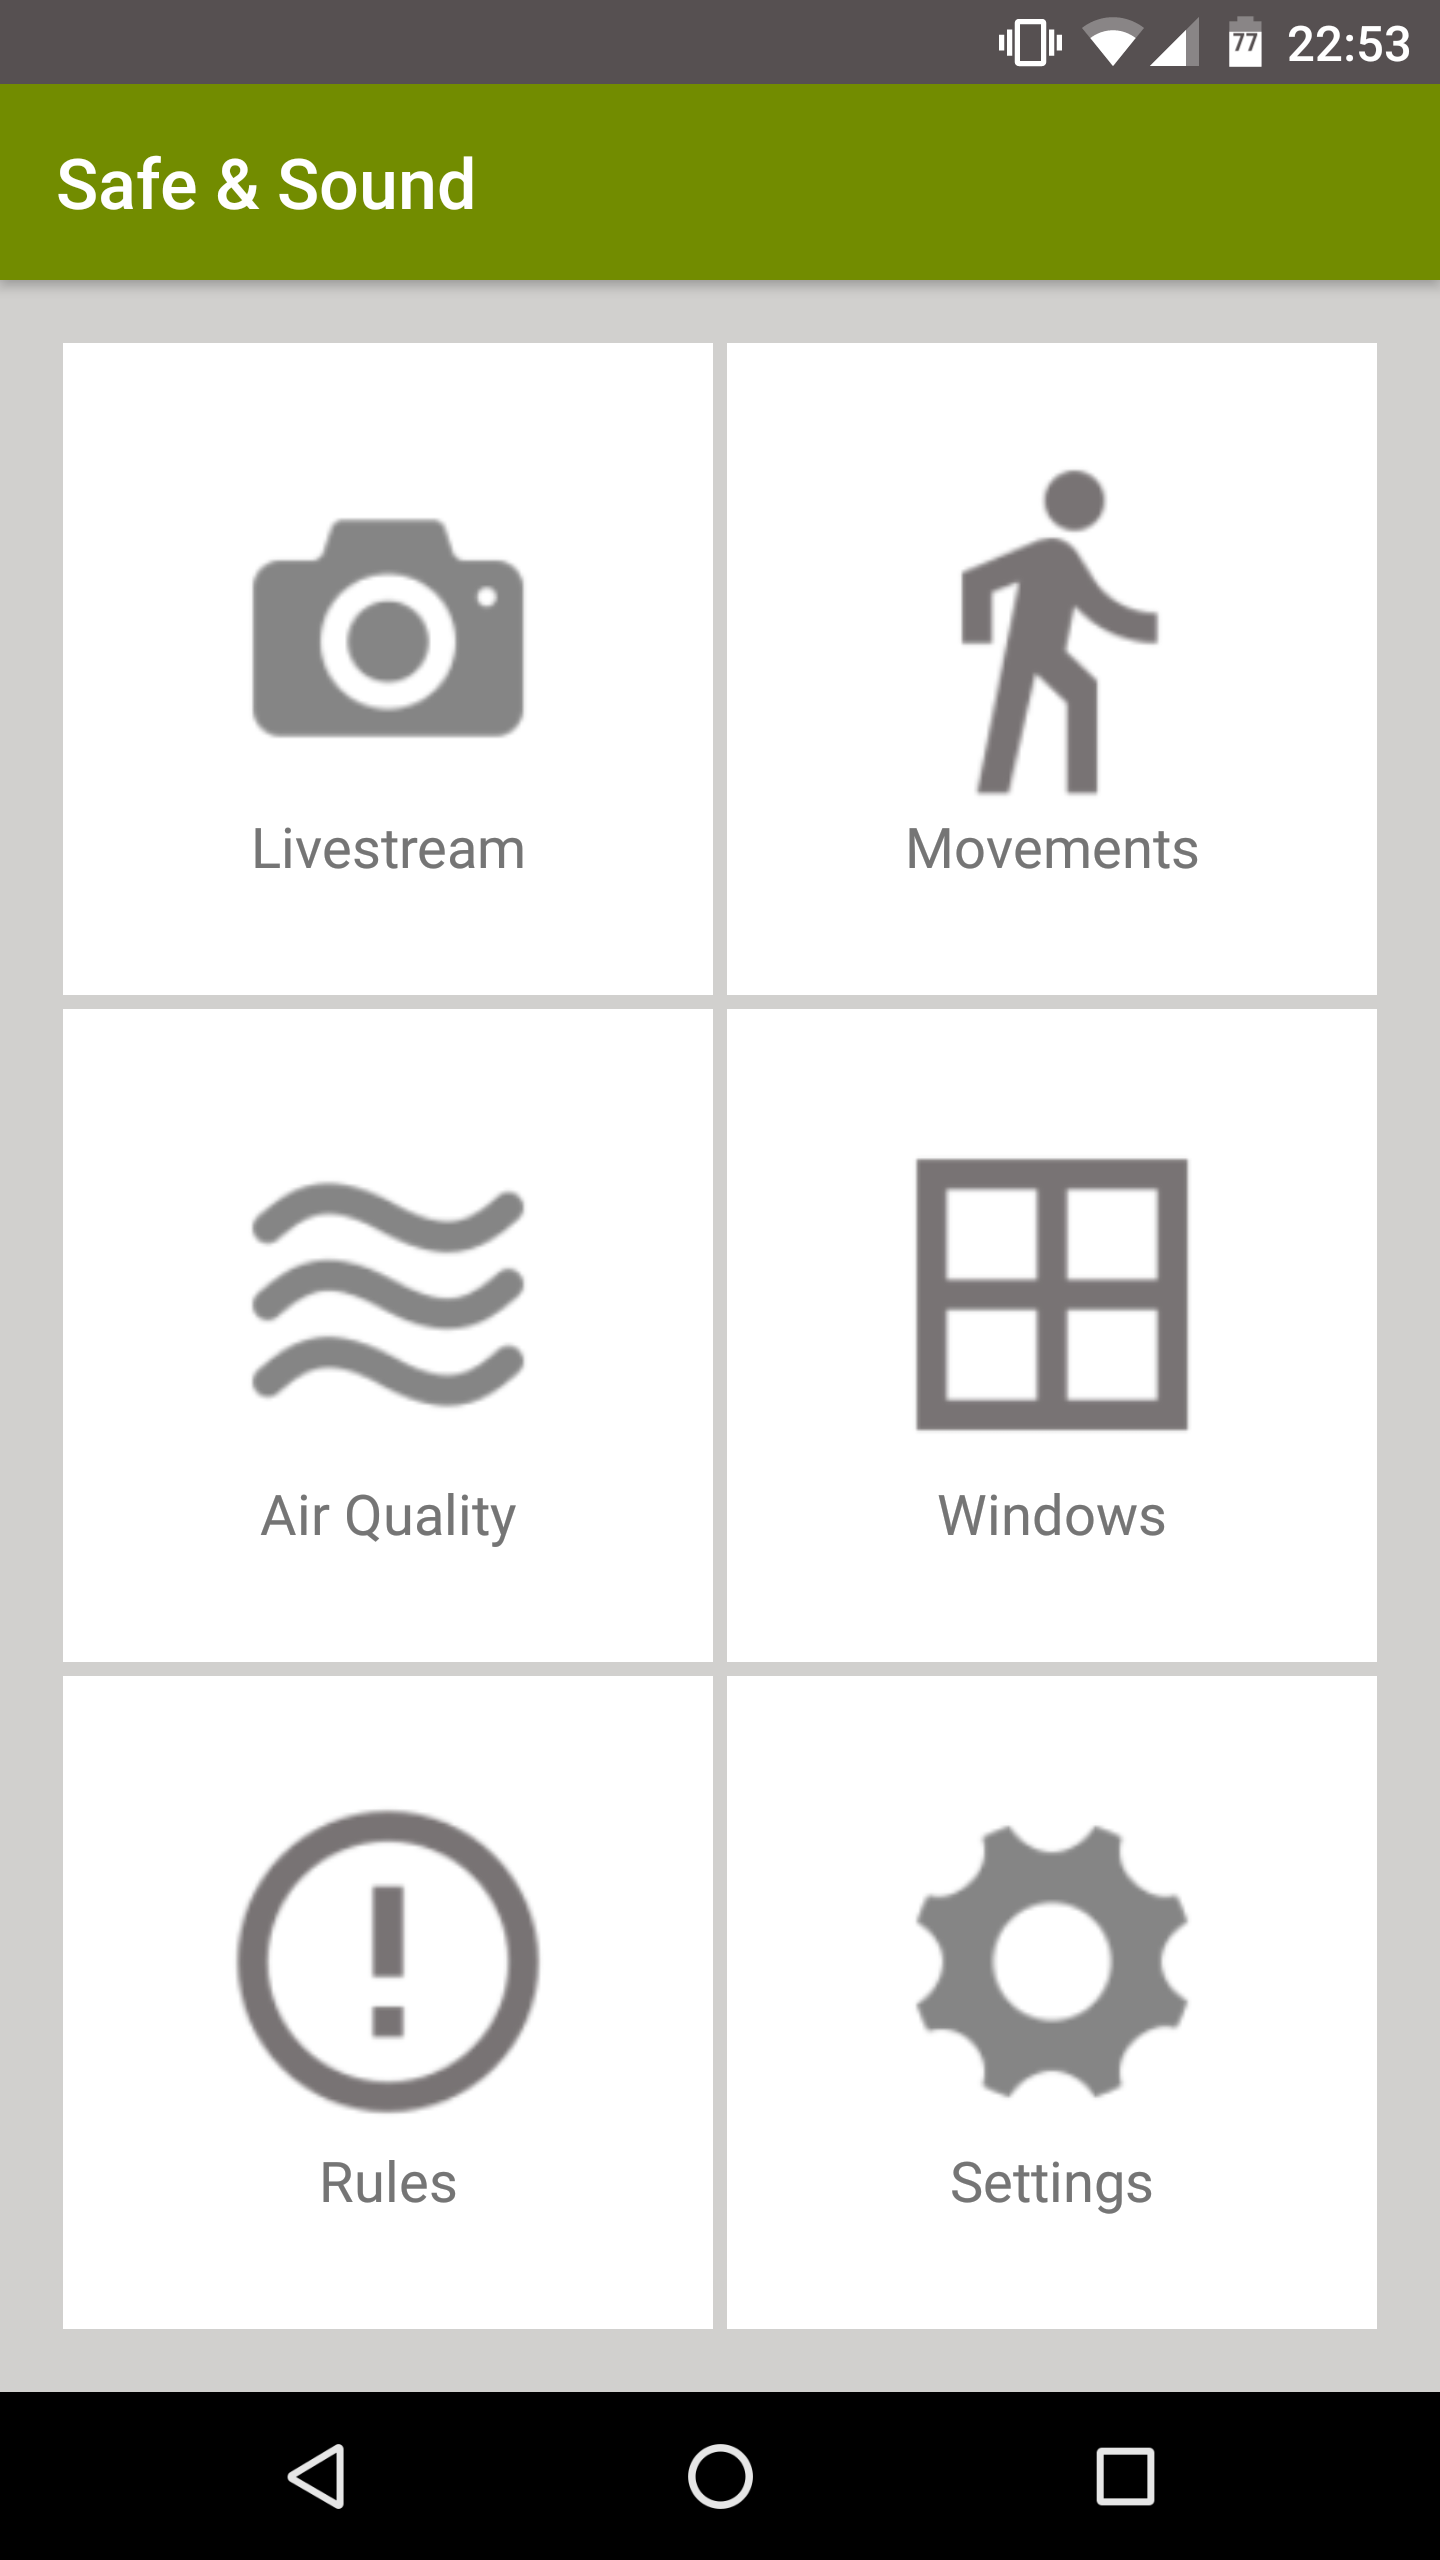
\includegraphics[scale=0.1]{images/appMain}
	\captionof{figure}{Startseite der App}
	\label{label:main}	
\end{minipage}
\begin{minipage}[c]{0.5\textwidth}
	\centering
	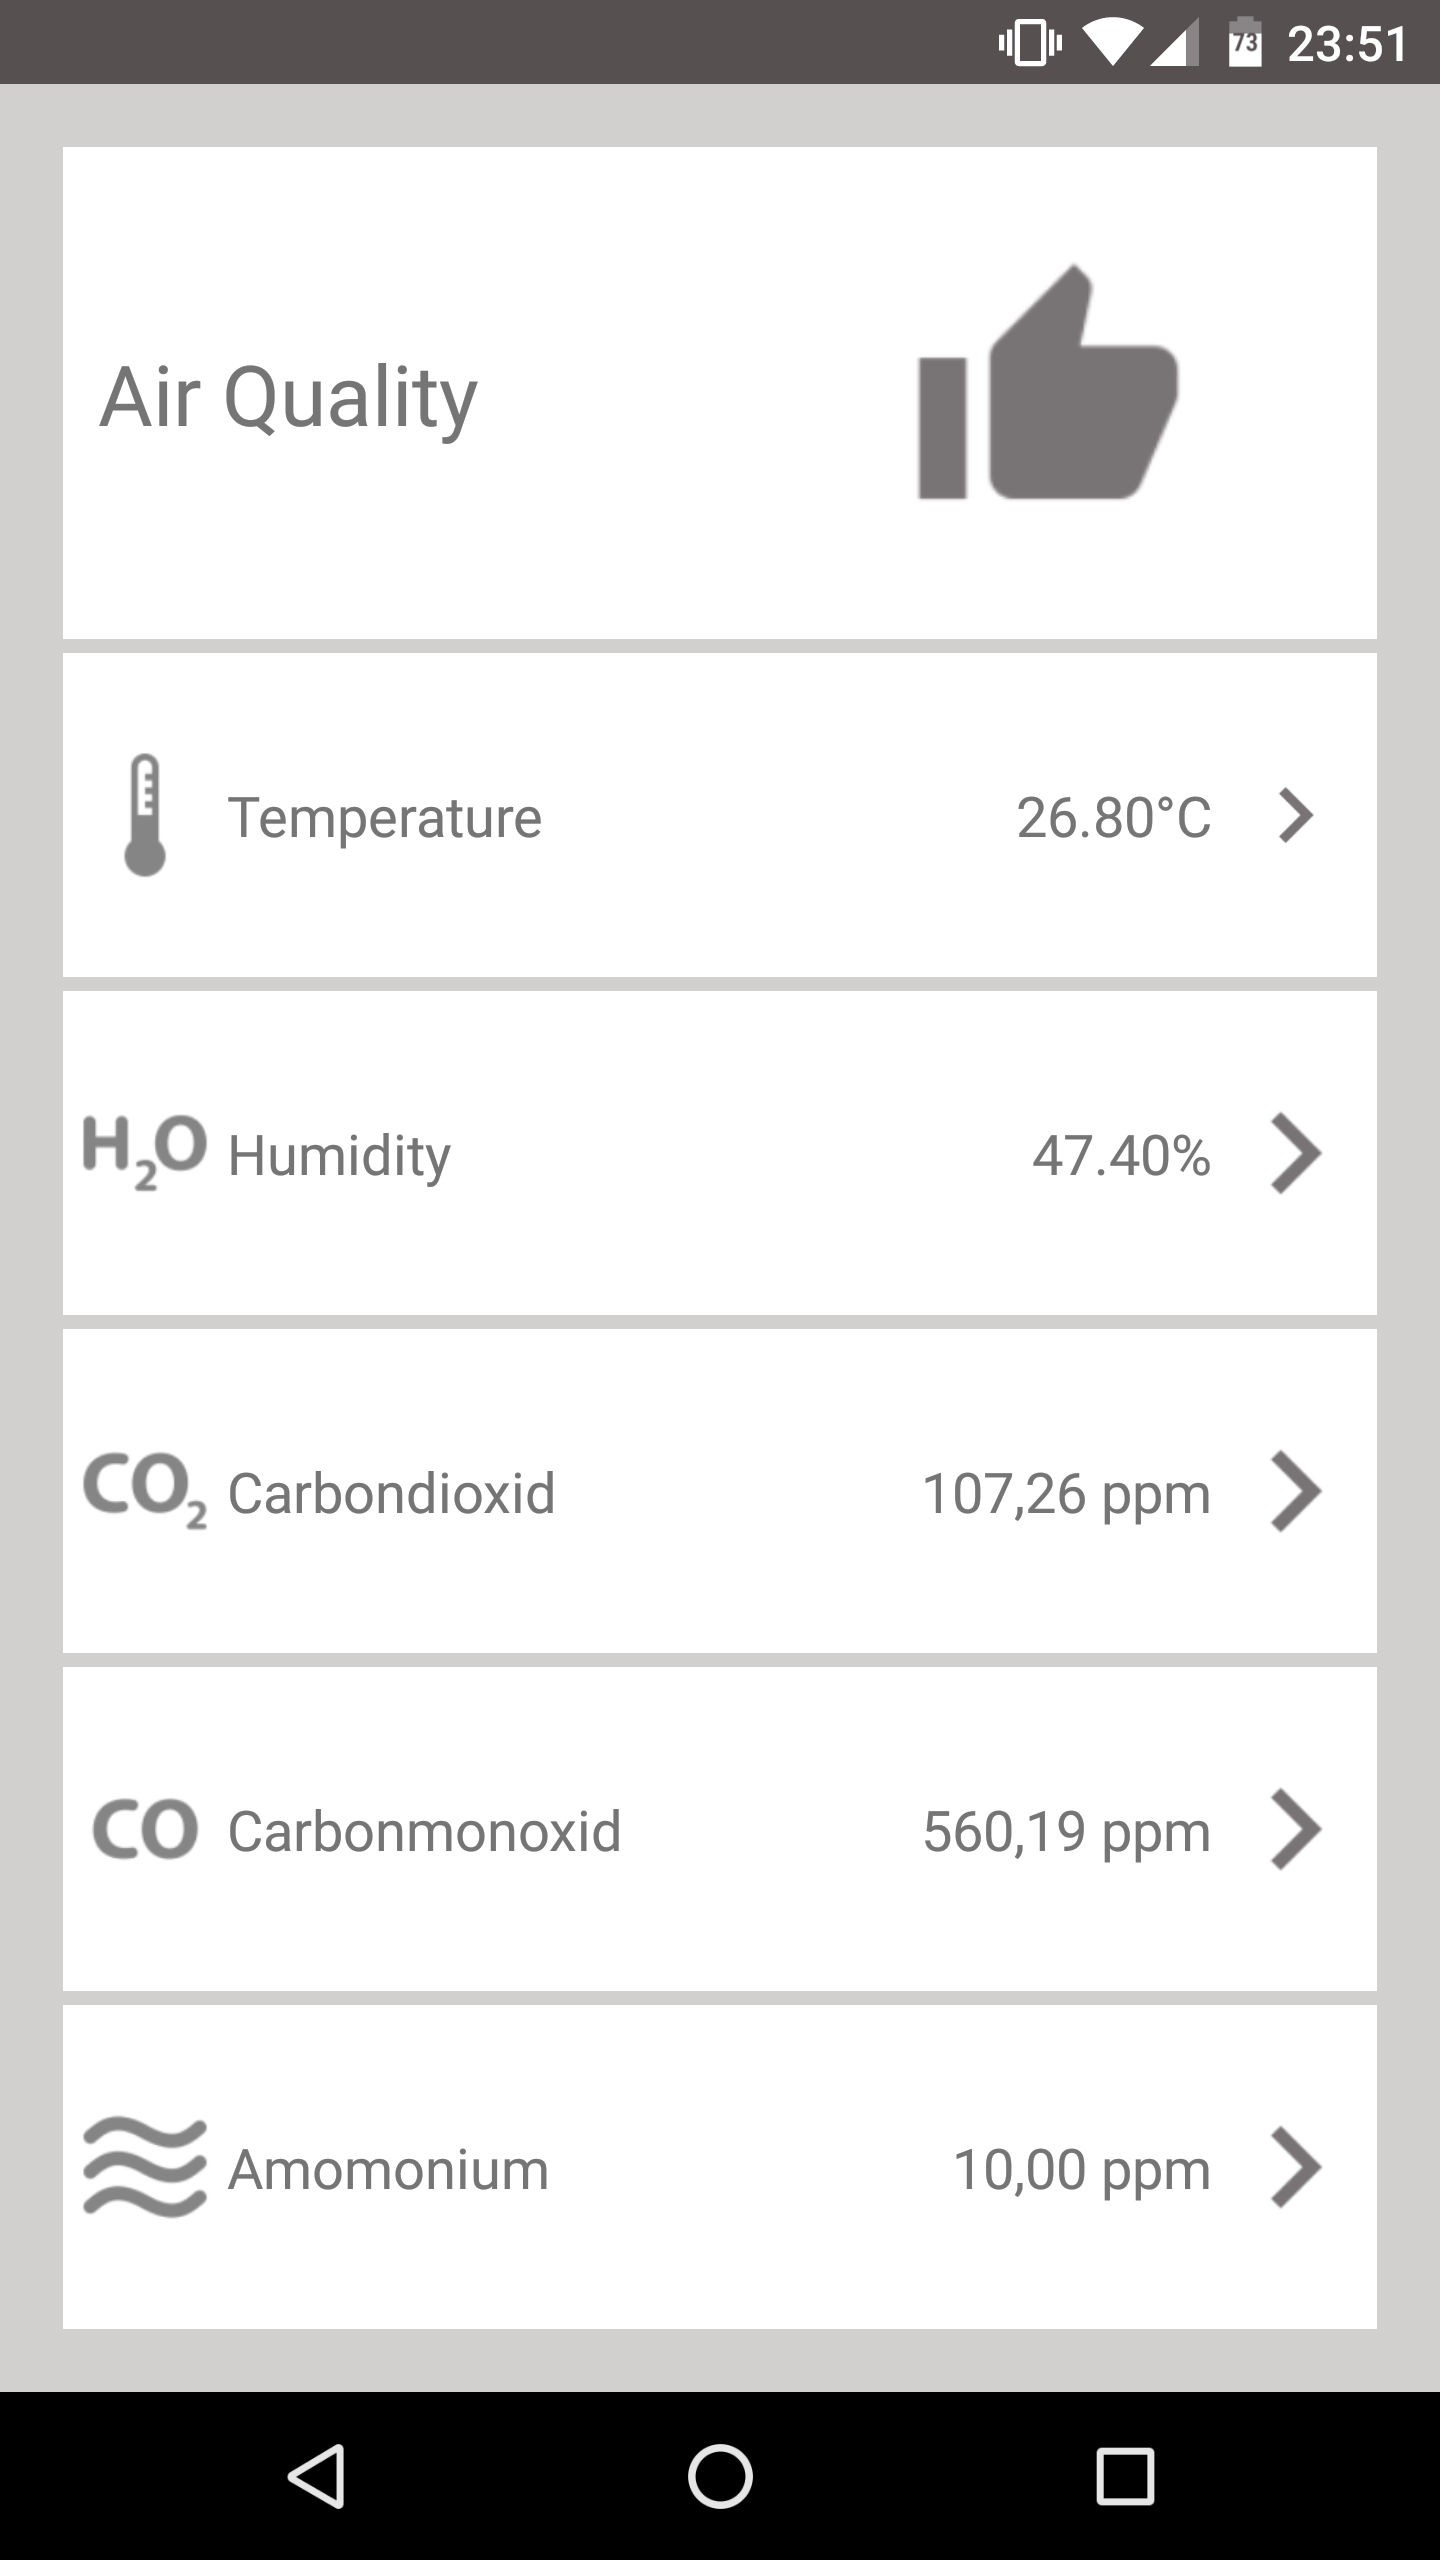
\includegraphics[scale=0.1]{images/airQuality}
	\captionof{figure}{AirQuality}
	\label{label:airquality}
\end{minipage}

Bevor dem Benutzer Daten angezeigt werden, muss dieser zuerst ein Intervall angeben. Dazu wird eine Eingabe über ein Start, sowie ein Enddatum notwendig. Wird nach erfolgreicher Auswahl des Intervalls der \enquote{Show Data} Button geklickt, siehe \autoref{label:tempVerlauf}, wird an den Webserver eine \ac{HTTP} Anfrage geschickt, die entweder für den angegebenen Zeitraum alle Temperatur und Luftfeuchtigkeitswerte oder MQ-135 Daten in einem \ac{JSON}-Array zurückliefert. 

\begin{figure}[h]
	\centering
	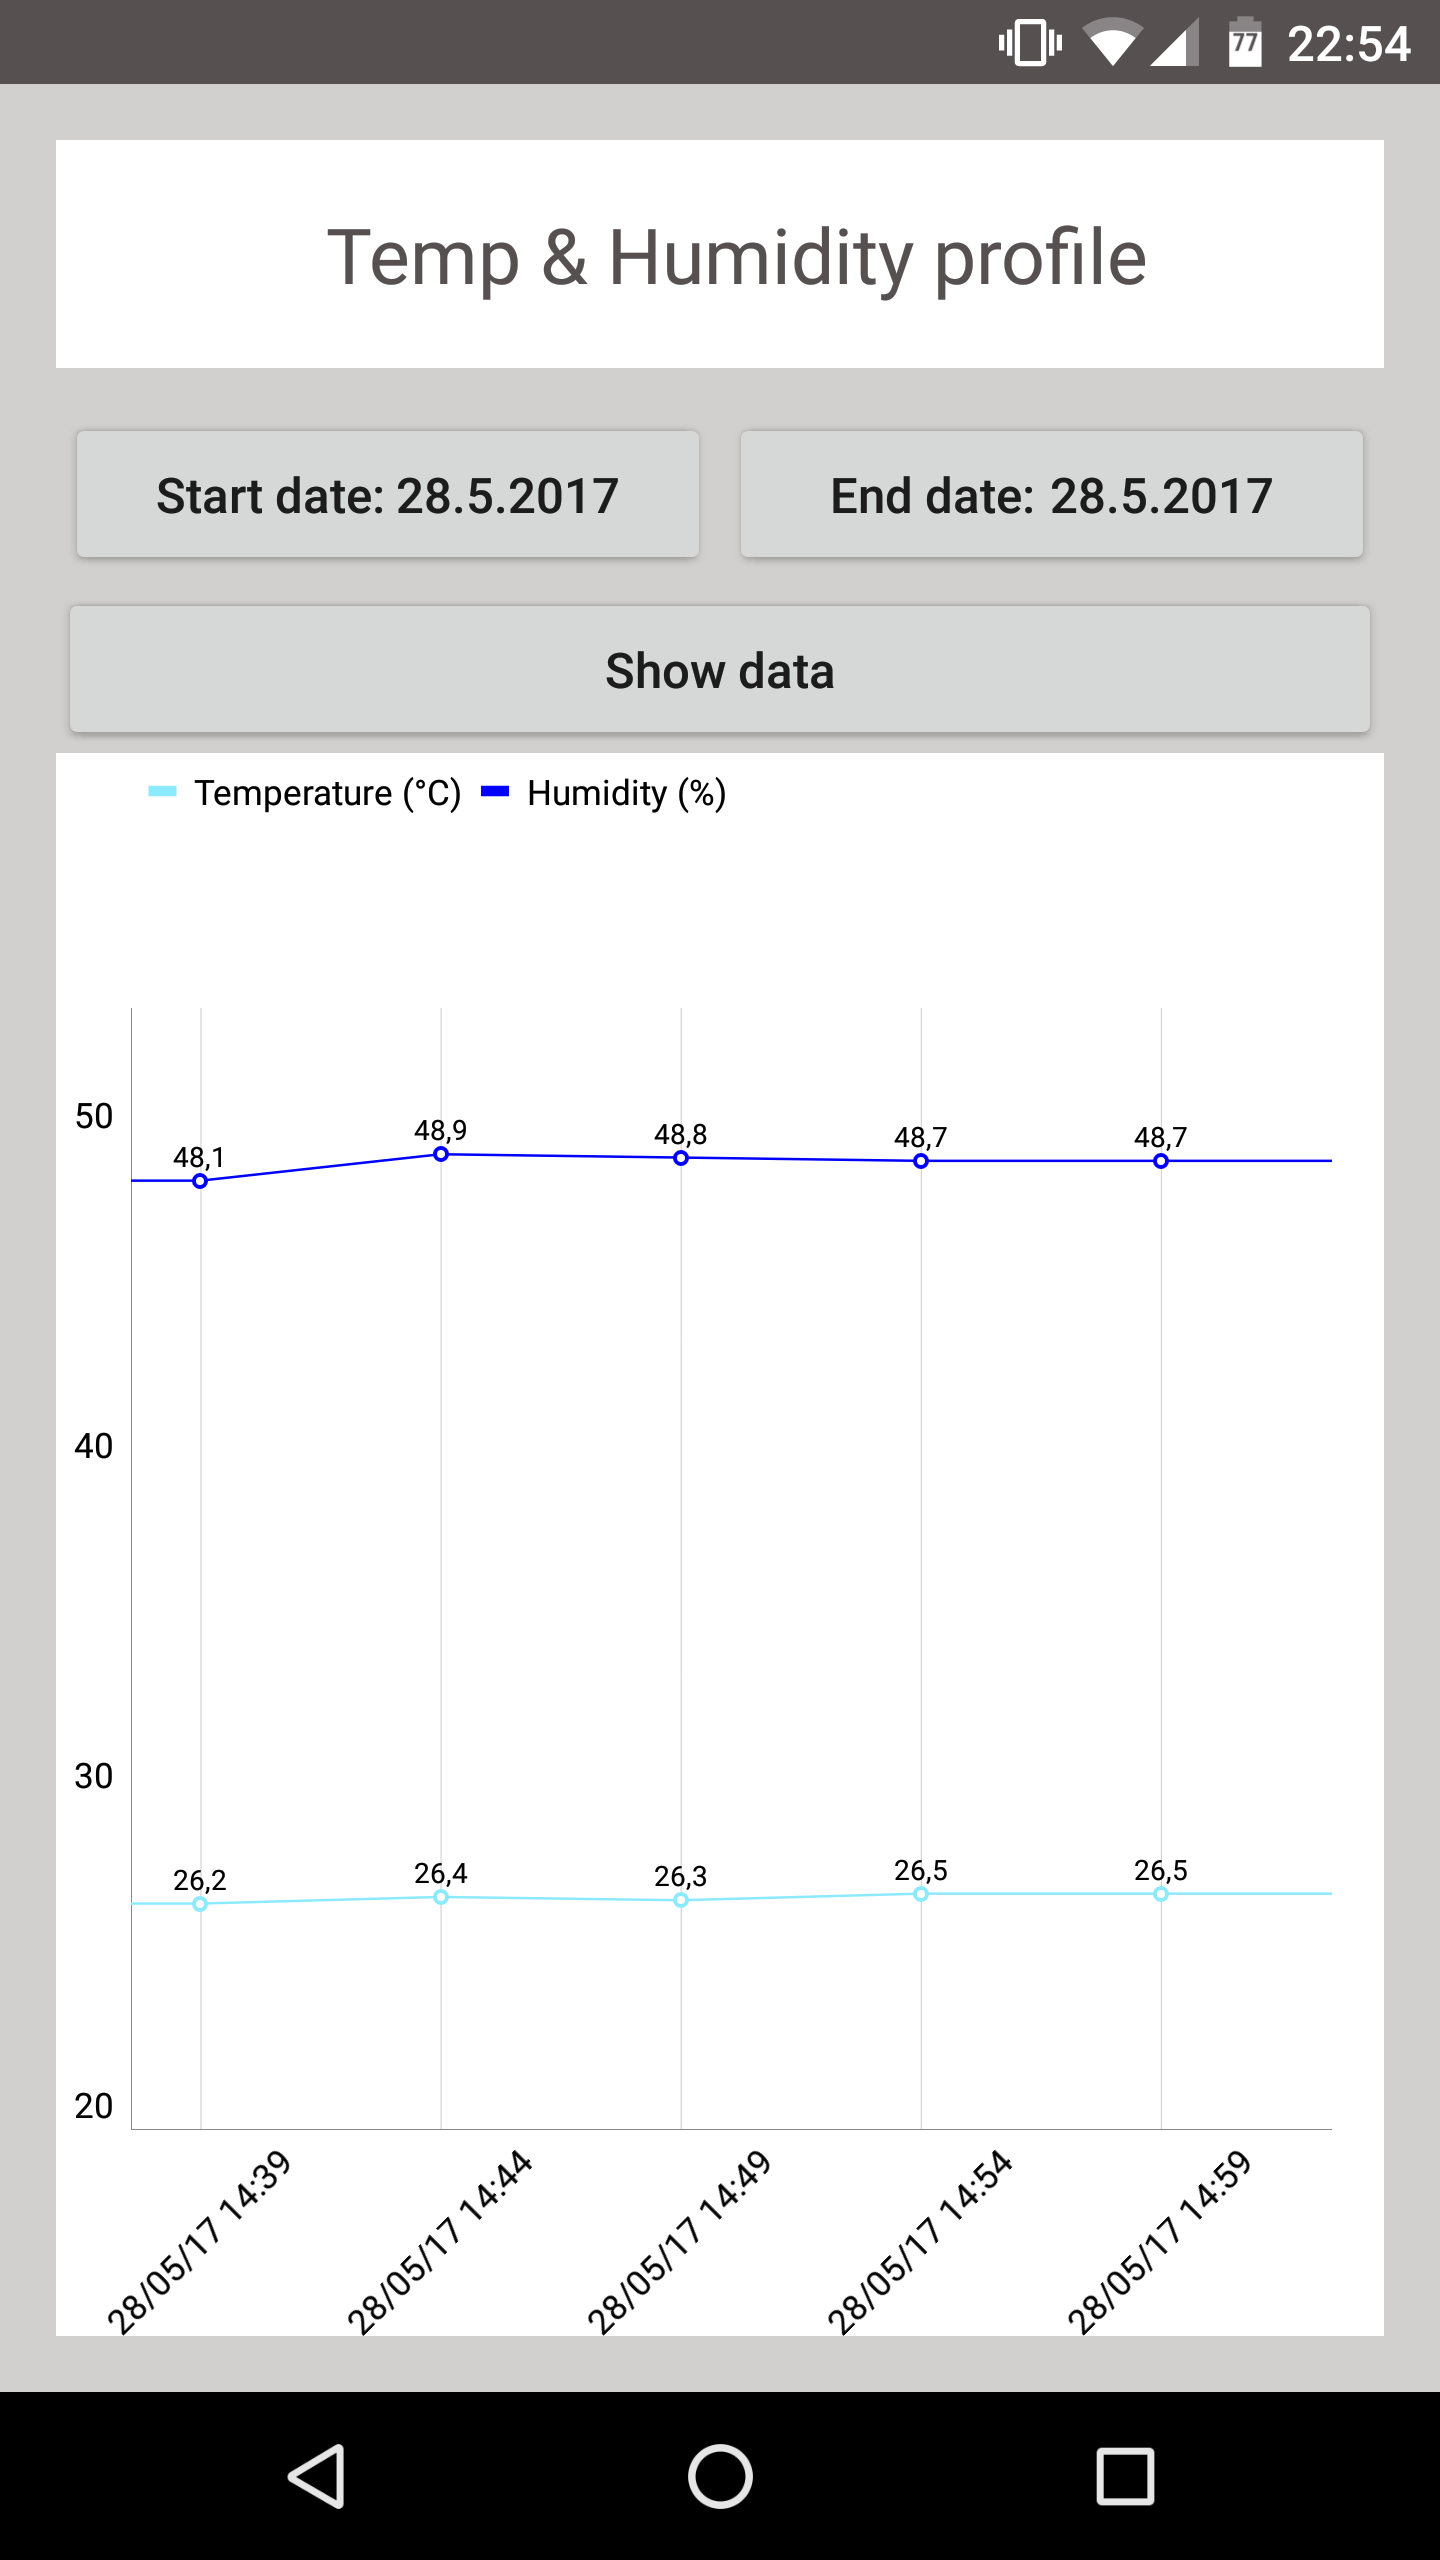
\includegraphics[scale=0.1]{images/appVerlauf}
	\caption{Diagramm Temperaturverlauf}
	\label{label:temVerlauf}
\end{figure}

\autoref{list:Array} zeigt als Beispiel das \ac{JSON}-Array auf, das vom Webserver als Response gesendet wird. 
\begin{lstlisting}[label=list:Array, caption={Beispiel: JSON Array}]
[
	{
		"id": 1184,
		"temperature": 25.8,
		"humidity": 47.9,
		"sensorid": "dht22",
		"timestamp": 1495971295531
	},
	{
		"id": 1185,
		"temperature": 25.8,
		"humidity": 47.9,
		"sensorid": "dht22",
		"timestamp": 1495971595619
	},
	{
		"id": 1186,
		"temperature": 25.9,
		"humidity": 47.8,
		"sensorid": "dht22",
		"timestamp": 1495971895672
	}
]
\end{lstlisting}

Damit nun die Daten in einem Liniendiagramm grafisch dargestellt werden können, ist es notwendig eine Bibliothek zum Visualisieren zu verwenden. Dabei viel die Auswahl auf \enquote{MPAndroidChart}\footcite{https://github.com/PhilJay/MPAndroidChart}. Allerdings gibt es viele verschiedene Bibliotheken, die als Open-Source-Software sich für diesen Zweck eignen.\\
Sobald die Webserver Response als String vorliegt, kann die in \autoref{label:getTem} aufgezeigte Funktion mit der Auswertung des Arrays beginnen. Dabei wird innerhalb der For-Schleife aus jedem \ac{JSON} Objekt der Temperatur- und Luftfeuchtigkeitswert ausgelesen. Die jeweiligen Werte müssen dann der entsprechenden ArrayListe als Entry übergeben werden (vgl. \autoref{label:getTem} Zeile 8ff). Ein Entry entspricht dabei einem Tupel aus zwei Werten für die x und y Koordinate.\\Nachdem alle Werte in der ArrayList \enquote{tempList} bzw. \enquote{humidityList} gespeichert sind, muss eine neue LineDataSet erzeugt werden, die passend zu den Werten noch eine Beschreibung hinzufügt. \\
Damit nun beide LineDataSets in einem Diagramm angezeigt werden können, wird in Zeile 22 eine neue ArrayListe definiert und bei LineDataSets hinzugefügt. Abschließend ein neues LineData Object erstellt und zurückgegeben werden. 

\begin{lstlisting}[label=label:getTem][h]
public LineData getTemHumDataForDiagramm(String s){

	List<Entry> tempList = new ArrayList<Entry>();
	List<Entry> humidityList = new ArrayList<Entry>();
	
	try{
		JSONArray jsonMainNode = new JSONArray(s);
		for(int i = 0; i < jsonMainNode.length(); i++){
			JSONObject jsonChildNode = jsonMainNode.getJSONObject(i);
			Float temperature = BigDecimal.valueOf(jsonChildNode.getDouble("temperature")).floatValue();
			tempList.add(new Entry((float)i, temperature));
			Float humidity = BigDecimal.valueOf(jsonChildNode.getDouble("humidity")).floatValue();
			humidityList.add(new Entry((float)i, humidity));
		}
	} catch (JSONException e){
		Toast.makeText(getApplicationContext(), "Error" + e.toString(), Toast.LENGTH_SHORT).show();
	}
	
	LineDataSet dataSetHum = new LineDataSet(humidityList,"Humidity (%)");	
	LineDataSet dataSetTemp = new LineDataSet(tempList,"Temperature (C)");
		
	List<ILineDataSet> dataSets = new ArrayList<ILineDataSet>();
	dataSets.add(dataSetTemp);
	dataSets.add(dataSetHum);
	
	LineData data = new LineData(dataSets);
	
	return data;
}
\end{lstlisting}

Damit nun die Daten im Diagramm angezeigt werden, müssen dem LineChart Objekt über die Methode \enquote{setData} die Daten übergeben werden. 
\begin{lstlisting}[label=list:showData]
LineChart chart = (LineChart) findViewById(R.id.chart);
LineData data = getTemHumDataForDiagramm(String s)
chart.setData(data)
\end{lstlisting}


	\chapter{Diskussion}

- JavaScript Engine hat eine Sicherheitslücke. --> Einfügen von JavaScript in Then Statement Feld möglich


	
\chapter{Ausblick}
Vorhersagen von WErten,
Analyse Verfahren entwickeln -> Gründe finden warum Raum nicht perfekt ist
Software soll über Motoren vorgänge automatisieren -> zu kalt automatisch fenster schließen
Lüften bis gute Werte erzielt werden

Die Anwendung könnte sich in Anbetracht in die Richtung einer Home Automation Steuerung entwickeln. Dafür müsste automatisierte Vorgänge im Raum gesteuert werden können. Beispielweise könnten als Use Case definiert werden, dass über die App basierend auf vom Benutzer definierten Regeln, Nachrichten gesendet werden, die beeinflussen, dass automatisch die Fenster geöffnet werden wenn es im Raum zu schlechte Gaskonzentrationswerte gibt.  
\\Ein weiteres Beispiel könnte die Vorhersage von Daten sein. Dazu müsste basierend aus den existierenden Daten ein Trend analysiert und ermittelt werden, sodass der Anwender mitgeteilt bekommt, wie der Temperaturverlauf in den nächsten Stunden wahrscheinlich sein wird. Um Vorhersagewerte treffen zu können, kann ein Datenmodell konzipiert werden und mit Hilfe eines Skriptes in der Sprache R ausgeführt werden. Die Vorhersagewerte werden in einer extra Spalte der Datentabelle eingefügt.\\
Die Vorhersagewerte bringen vor allem dann einen Mehrwert, wenn die Sensoren zeitweise ausfallen. Über die Vorhersage können dann weiterhin Handlungsvorschläge getroffen werden. Die Pfleger können sich weiterhin auf das System verlassen.\\
Um den Mehrwert der Applikation zu steigern, sollte der Regel Engine eine Timer-Funktion hinzugefügt werden. Durch die Timer-Funktion können Regel hinzugefügt werden auf Basis von Zeitintervallen. Ein Anwendungsfall für den Nutzen eines Timers ist die Statusänderung des Fensters. Ein Nutzer möchte nicht zwingend benachrichtigt werden, wenn ein fenster geöffnet ist, sondern viel mehr wenn ein Fenster länger als einen gegebenen Zeitintervall geöffnet ist. Durch die Implementierung der Rule Engine mit einem JavaScript Interpreter ist das Hinzufügen eines Timers möglich. JavaScript bietet Bibliotheken für Timer Implementierungen an.\\
	
	\clearpage

	% Literaturverzeichnis
	\cleardoublepage
	\printbibliography

	% Glossar
	\printglossary[style=altlist,title=\langglossar]
	
	% sonstiger Anhang
	\clearpage
	\appendix
	% !TeX root = ../dokumentation.tex

\addchap{\langanhang}
\renewcommand{\thefigure}{A\arabic{figure}}

\setcounter{figure}{0}

\begin{lstlisting}[label=list:MQClass, caption={Auswertung der MQ-Sensorwerte}]
import time
import math
from MCP3008 import MCP3008

class MQ():

	# define which analog input channel you are going to use (MCP3008)
	MQ_PIN                       = 0        
	# define the load resistance on the board, in kilo ohms
	RL_VALUE                     = 5        
	# RO_CLEAR_AIR_FACTOR derived from the chart in datasheet
	RO_CLEAN_AIR_FACTOR          = 3.57    
	
	CALIBARAION_SAMPLE_TIMES     = 500       
	CALIBRATION_SAMPLE_INTERVAL  = 100      
	READ_SAMPLE_INTERVAL         = 50       
	READ_SAMPLE_TIMES            = 5        
	
	GAS_CO2                      = 0
	GAS_CO                       = 1
	GAS_NH4                      = 2
	
	def __init__(self, Ro=4, analogPin=0):
	self.Ro = Ro
	self.MQ_PIN = analogPin
	self.adc = MCP3008()
	
	#Sensore specific lien
	self.CO2Curve = [1,0.352,-0.331]   
	self.COCurve = [1,0.462,-0.258]  
	self.NH4Curve =[1,0,423,-0.423]   
	
	print("Calibrating...")
	self.Ro = self.MQCalibration(self.MQ_PIN)
	print("Calibration is done...\n")
	print("Ro=%f kohm" % self.Ro)
	
	
	def MQPercentage(self):
	
		val = {}
		read = self.MQRead(self.MQ_PIN)
		val["CO2"]  = self.MQGetGasPercentage(read/self.Ro, self.GAS_CO2)
		val["CO"]   = self.MQGetGasPercentage(read/self.Ro, self.GAS_CO)
		val["NH4"]  = self.MQGetGasPercentage(read/self.Ro, self.GAS_NH4)
		return val
	
	def MQResistanceCalculation(self, raw_adc):
		if(raw_adc != 0):
		return float(self.RL_VALUE*(1023.0-raw_adc)/float(raw_adc));            
		else:
		return 0.0;
	
	def MQCalibration(self, mq_pin):
		val = 0.0
		count = 0
		for i in range(self.CALIBARAION_SAMPLE_TIMES):          
			helper = self.MQResistanceCalculation(self.adc.read(mq_pin))
			#handle errors		
			if(helper != 0.0):
			val += helper
			count = count +1
			time.sleep(self.CALIBRATION_SAMPLE_INTERVAL/1000.0)
	
		val = val/count                                         
	
		val = val/self.RO_CLEAN_AIR_FACTOR                     
		# according to the chart in the datasheet 
		return val;
	
	
	def MQRead(self, mq_pin):
		rs = 0.0
		
		for i in range(self.READ_SAMPLE_TIMES):
		rs += self.MQResistanceCalculation(self.adc.read(mq_pin))
		time.sleep(self.READ_SAMPLE_INTERVAL/1000.0)
		
		rs = rs/self.READ_SAMPLE_TIMES
		
		return rs
	
	def MQGetGasPercentage(self, rs_ro_ratio, gas_id):
		if ( gas_id == self.GAS_CO2 ):
			return self.MQGetPercentage(rs_ro_ratio, self.CO2Curve)
		elif ( gas_id == self.GAS_CO ):
			return self.MQGetPercentage(rs_ro_ratio, self.COCurve)
		elif ( gas_id == self.GAS_NH4 ):
			return self.MQGetPercentage(rs_ro_ratio, self.NH4Curve)
		return 0

	def MQGetPercentage(self, rs_ro_ratio, pcurve):
		return (math.pow(10,( ((math.log(rs_ro_ratio)-pcurve[1])/ pcurve[2]) + pcurve[0])))
	

\end{lstlisting}
\begin{figure}
	\centering
	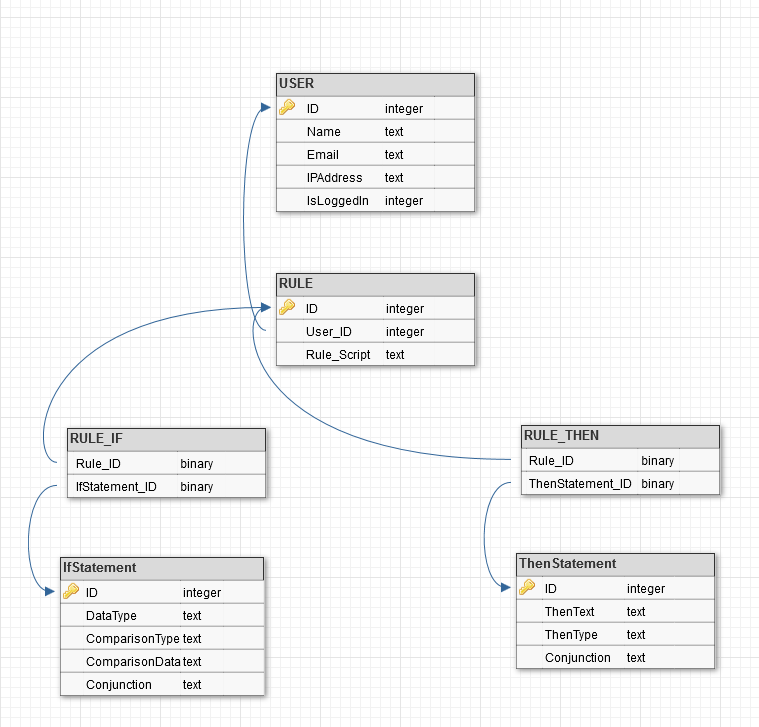
\includegraphics[width=1\textwidth]{images/DBSchema.png}
	\caption{Datenbank Schema der Android SQLite Datenbank}
	\label{fig:androiddbschema}
\end{figure}
	
\end{document}
